\documentclass[a4paper,11pt,english]{article}
\usepackage[english]{babel}
\usepackage{lmodern}
\usepackage[T1]{fontenc}
\usepackage[utf8]{inputenc}
\usepackage{graphicx}
\usepackage{amsmath, amsthm, amssymb, amsfonts}
\usepackage{verbatim}
\usepackage[skip=2pt,font=small, margin=1cm]{caption}
\usepackage{url}
\usepackage[round]{natbib}  
\usepackage{hyperref}
\usepackage{subcaption}
\usepackage{float}
\usepackage{rotating, threeparttable, booktabs} % fjern ellers
\usepackage{color}    %fjern ellers
\usepackage{dcolumn}  %fjern ellers
\usepackage{enumerate}
\usepackage[]{algorithm2e}	
\pagenumbering{roman} 
\setlength{\parindent}{0pt}
\newcommand{\E}{\mathbb{E}}

\begin{document}
	
	\tableofcontents
	\listoffigures
 	\listoftables
  	\pagebreak
	\pagestyle{empty}
	\abstract{\noindent 

	This thesis mainly focus on practical applications of rigorous mathematical modelling and financial engineering of the Hamiltonian Markov 
	Regime Switching models. 
	
	
	In this thesis, we shall consider a stock's volatility estimation  
	on practical implementation of the Hamilton and Susmel model that models the fucking financial times series that
	subject to sudden discrete changes in regimes. 
	
	modeling of the dynamic structure of volatility
	
	modelling ARCH(1) stochastic process for financial time series of  in combination with following three 
	models, namely, an ARCH(1), a GARCH(1,1) and a Markov regime switching model. 

	More precisely, we attempt to use various modern numerical solutions, techniques and tools to generate the respective answers.
	
	MS-ARCH($p,q$) has become a growing area of interest	
	
	I am looking at econometric models of a nonstationary times series that is governed by sudden discrete changes in regimes.
	
	Fubini, in process,\ldots I use MCMC methodology and Bayesian Inference to estimate a vector of unknown parameters for 
	stochastic ARCH process Markov Switching Model. I use modern statistical computing to simulate based on Gibbs Sampling.  I maximize convex 
	likelihood for ARCH(1) model.~\vspace{0,3cm}

	The dynamic structure of volatility 	
		
	\vspace{0,3cm}	
		
	%Fubini, fix me later!..
HMMs and 
	In this thesis, we present the basic concepts, theory and associated academical approaches and practical implementation of algorithms for hidden 
	Markov models, time series and 
	%autoregressive hidden Markov models. I have also built a bivariate autoregressive hidden Markov model on the temperature data from the Pacific 
	%Ocean to understand the mechanism of El Nino. The parameters and the state path of the model are estimated through the Segmental K-mean algorithm 
	%and the state estimations of the autoregressive hidden Markov model have been compared with the estimations from a conventional hidden Markov model. 
	%Overall, the results confirm the strength of the autoregressive hidden Markov models in the El Nino study and the research sets an example of 			
	%ARHMM's application in the meteorology. \\
		\vspace{0,3cm}	
	
	\noindent \textit{Keywords and phrases:} \textsc{time series modelling; autoregressive conditional heteroscedasticity; arch models; markov chain monte 
	carlo; mcmc; markov chain methods of sampling; gibbs sampling; metropolis algorithm, metropolis hastings algorithm; metropolis within gibbs algorithm; 
	statistical computing; modern statistics parameter estimation; time varying transition probabilities; hidden markov models; hmm; regime changes; markov 
	regime switching models; msm; mrsm; markov regime-switching arch model; stochastic simulation; probabilistic programming framework; computational 	
	statistics; stock prices; stock volatility; machine learning; nonstationary; nonlinear filtering; bayesian statistics; bayesian inference; bayesian 
	philosophy; bayesian data analysis; bayesian computations.}}
	
	
%	\pagebreak
	\pagebreak	
	\clearpage
	\setcounter{page}{1}
	\pagenumbering{arabic}		
	\pagestyle{plain}

	
	%##############################################################################################################################################		
	\section{Introduction}
	%##############################################################################################################################################
	
	The theory that we introduce throughout the thesis, will be illustrated through an application on on two publicly traded stocks with daily 
	observations. \vskip 0.3cm 	

	I want to take a closer look at, one popular and widely used approach in academia to modelling volatility of various economic and financial time
	series (such as, stock prices, an empirical analysis of a business cycle, etc\ldots), which is Autoregressive Conditional Heteroscedasticity Model's
	specifications and theoretical aspects, that was introduced by~\citep{engle82}; cf., inter alia~\citep[p.~308]{hamiltonsusmel}. \vskip 0.3cm 
	
	to modelling volatility of various \vskip 0.3cm 


	%This thesis has a modular structure. I present various mathematical theory and formal techniques, though we will not use it all in our practical 
	%implementation. 

	%when financial series undergo sudden changes in embedded discrete states; Markov switching in variance 	
	
	The rest of the thesis is organized in the following way. Section 1 sets out the basic Fubini model. In section 2 we will present a general 
	introduction 
	of time series models,\ldots Followed by discussions of Fubini in section 3 focuses on the  FUBINI,\ldots.. Then, in section 4  
	FUBINI,\ldots application of a conventional hidden Markov model in stocks' data performed and related experimental results discussed in 
	section 5. Finally, in section 6, we provide a summary discussion. In section 7, we provide an application of the 
	proposed methods to financial time series for two stocks. Finally, in Section FUBINI we discuss issues of the practical implementation.		
	%writte; focus; describe; present; explain; take a closer look at; introduce; provides an overview of FUBINI; discusses the role FUBINI
	%the methodology and results presented in section FUBINI; ..., and we offer some concluding remarks in Section FUBINI
	%in a more formal way
	
	
			

	%#########################################################################################################################
	\section{Financial Time Series}
	%#########################################################################################################################
		
		Fubini, in process\ldots I am interested in analysis of financial time series.
		
		%###########################################################################################################
		\subsection{Fubini}
		%###########################################################################################################
		
		Fubini, in process\ldots

			%###########################################################################################################
			\subsubsection{Fubini}
			%###########################################################################################################
			
			Fubini, in process\ldots
		
		%#########################################################################################################################
		\subsection{Conditional Heteroscedastic Models}
		\label{subsec:arch}
		%#########################################################################################################################

		The absolutely first econometric model that was successful to modify the traditional unrealistic assumption about a constant one-period forecast 
		variance, was proposed by \citep{engle82}. Robert Engle in his paper introduced a new class of stochastic processes, the so-called 
		autoregressive conditional heteroscedastic (ARCH) processes. He has also provided specifications and systematic framework for a setup of dynamic 
		volatility modelling. Later,~\citep{bollerslev} characterized a general class of ARCH as generalized ARCH (GARCH($m,n$)). 
				
		The ARCH-effects, which is also known as the conditional heteroscedasticity, is a well-known phenomenon. It represents tendency of volatility 
		clustering of a stock market data. Such that, a large(small) change has a tendency to replicate itself, such that it is followed by somewhat 
		larger(smaller) relative changes. Now, ARCH and GARCH models have such an ability to model this phenomenon. These kind of models widely used and in 
		variety of academic papers and is a popular approach in financial applications~\citep{canarella}.

						
			%###########################################################################################################
			\subsubsection{Properties of ARCH($m$) Models}
			%###########################################################################################################
			
			I begin our study with ARCH($m$) models. Here $m$ denotes the order of ARCH process, which is, the number of lagged states that 
			matter of interest in a specific model, see more~\citep[p.~115, p.~119]{tsay},~\citep[p.~308]{hamiltonsusmel} and the code comments in SWARCH 
			Maxseek function. 

			The fundamental structure of ARCH models assumes that a \emph{shock} $a_t$ (also known as an~\emph{innovation} or~\emph{current error term}) is 
			serially uncorrelated process with mean zero, and variance that depends on the sum of squared recent past 
			shocks~$\left\{a^2_{t-i} \right\}^m_{i=1}$. More specifically, in ARCH($m$) model we assume that a variable $a_t$ at time $t$ is governed by
			\begin{equation*}
				a_t = \sigma_t \epsilon_t,
			\end{equation*}
			such that, the conditional variance of $a_t$ depends on a quadratic function of its past realizations 
			\begin{eqnarray} \label{eq:quadratic}
				\sigma_t^2 &=&  \alpha_0 + \alpha_1 a^2_{t-1} + \alpha_2 a^2_{t-2} + \cdots + \alpha_{m-1} a^2_{t-m-1}  + \alpha_m a^2_{t-m}  \\
						 &=& \alpha_0 + \sum_{i=1}^{m} \alpha_i a^2_{t-i},
			\end{eqnarray}								
			where $\left\{\epsilon_t \right\}_{t=1}^T$ is a sequence of Gaussian white noises\footnote{\emph{innovations} in most 
			econometric models modelled by standard normal distribution, though~\citep{hamiltonsusmel} in their paper discuss the advantage of Student t 
			distribution}, and 
			\begin{eqnarray*}
			\underline{\alpha} = (\alpha_0, \alpha_1, \ldots, \alpha_{t-m-1}, \alpha_m)
			\end{eqnarray*}
			is a vector of unknown parameters, with $\alpha_0 > 0 \text{ and } \alpha_i\geq 0$ conditions for $i > 0$. As a result, this guarantees the 
			conditional variances $\sigma_t^2$  to be positive for all $t$.~\vspace{0,3cm}	
			
			The simple first-order model ARCH(1) can be represented, as the set of following equations
			\begin{eqnarray} \label{eq:arch1}
			a_t = \sigma_t \epsilon_t, \text{ } \sigma_t = \sqrt[]{\alpha_0 + \alpha_1 a^2_{t-1}}, \text{ }	\sigma_t^2 = \alpha_0 + \alpha_1 a^2_{t-1}, 
			\end{eqnarray}
			where $\alpha_0 > 0$, $\alpha_1 \geq 0$, $\epsilon_t$ is independent of the past, and $\sigma_t$ is known function value of the prior 
			information at time $t-1$.   
			
			First, the unconditional mean of $a_t$ remains zero, because 
			\begin{eqnarray*}
				E(a_t) &=& E\left[ E(a_t | F_{t-1}) \right] = E\left[ E(\sigma_t \epsilon_t | F_{t-1}) \right] \\
				       &=& E\left[ \sigma_t \right] E\left[ (\epsilon_t | F_{t-1}) \right]  = E\left[ \sigma_t \right]  E(\epsilon_t) 
				       = E\left[ \sigma_t \right]  0 = 0.
			\end{eqnarray*}						
			
			Second, assuming that $a_t$ is a stationary process with $E(a_t) = 0$, $Var(a_t) = E(a^2_t) = Var(a_{t-1}) = E(a^2_{t-1})$, we can obtain
			the \emph{unconditional variance} of $a_t$
	
			\begin{eqnarray*}
	         Var(a_t) &=& E(a^2_t) = E\left[ E(a^2_t | F_{t-1}) \right] = E\left[ E(\sigma_t^2 \epsilon_t^2 | F_{t-1}) \right]   \\
			          &=& E\left[\sigma_t^2 E(\epsilon_t^2) \right] = E\left[1 \sigma_t^2 \right] = E\left[\alpha_0 + \alpha_1 a^2_{t-1} \right] \\
			    	  &=&	\alpha_0 + \alpha_1 E\left[a^2_{t-1} \right] = \alpha_0 + \alpha_1 E\left[a^2_t \right] \\
			    	  &=& \alpha_0 + \alpha_1 Var(a_t),
			\end{eqnarray*}
			here it is very interesting to observe, that the left hand side of the equation, equals the right hand side. Where, the $rhs$ is a sum of one 
			constant, and a product of another constant and a $lhs$' value. If $\alpha_1  \geq 1$ then $ Var(a_t) < Var(a_{t-1})$, which means ascending 
			variance. Therefore, the inequality remains true, as long as $\alpha_1$ constraint is less then $1$. Solving, with respect to the unconditional 
			variance, we can obtain 
			\begin{eqnarray*}
				Var(a_t) &=& \alpha_0 + \alpha_1 Var(a_t) \Leftrightarrow  \\ 
				\alpha_0 &=& Var(a_t)(1-\alpha_1)  \Leftrightarrow\\
				Var(a_t)&=& \frac{\alpha_0}{1 - \alpha_1}.  
			\end{eqnarray*} 
			
			Third, and this is especially in some financial applications, we may be interested in the kurtosis $m_4$ of $a_t$.
			Hence, there are some additional constraints that $\alpha_1$ must follow. Assume $m_4 = E(a_t^4) = E(a_{t-1}^4)$ 
			is finite. By applying the normality assumption of $\left\{ \epsilon_t \right\}$ in eqn~\ref{eq:arch1}, we get
			\begin{eqnarray*}
				m_4 &=& E(a_t^4) = E\left[E(a^4_t | F_{t-1}) \right] =  E\left[E(\sigma^4_t \epsilon^4_t | F_{t-1})\right]         \\
				 &=& E\left[\sigma^4_t E(\epsilon^4_t ) \right] = E\left[3 \sigma^4_t \right] = 3 E\left[ (\sigma^2_t)^2 \right]   \\ 
 				 &=& 3 E\left[ (\alpha_0 + \alpha_1 a^2_{t-1})^2 \right]                                                           \\
				 &=& 3 E\left[ \alpha_0^2 + 2 \alpha_0 \alpha_1 a^2_{t-1} + \alpha_1^2 a^4_{t-1} \right]                           \\
				 &=& 3 (\alpha_0^2 + 2 \alpha_0 \alpha_1 E\left[a^2_{t-1}\right]  + \alpha_1^2 E\left[a^4_{t-1}\right] )           \\
				 &=& 3 (\alpha_0^2 + 2 \alpha_0 \alpha_1 Var(a^2_t) + \alpha_1^2 E\left[a^4_t\right])                              \\
				 &=& 3 (\alpha_0^2 + 2 \alpha_0 \alpha_1 \frac{\alpha_0}{1-\alpha_1} + \alpha_1^2 m_4)                             \\
				 &=& 3 \alpha_0^2\Bigl(1 + 2  \frac{\alpha_1}{1-\alpha_1}\Bigr) + 3\alpha_1^2 m_4                              	   \\
				 &=& 3 \alpha_0^2\Bigl(\frac{1+\alpha_1}{1-\alpha_1}\Bigr) + 3\alpha_1^2 m_4,
			\end{eqnarray*}
			where we can see, that the $rhs$ can only be equal $lhs$, if $3 \alpha_1^2 < 1 \Leftrightarrow \alpha_1 = \sqrt{1/3}$. Otherwise, the fourth 
			moment will be growing. Consequently, solving with respect to $m_4$, we get the following result
			\begin{eqnarray*}
				m_4 (1 - 3 \alpha_1^2) &=&  \frac{3 \alpha_t^2 (1+\alpha_1)}{(1-\alpha_1)}\text{ }\text{ }\text{ } \Leftrightarrow  \\
				m_4 &=& \frac{3 \alpha_0^2(1+\alpha_1)}{(1-\alpha_1)(1 - 3\alpha^2_1)}. 
			\end{eqnarray*}
			The $m_4$ is always positive, that is why the $\alpha_1$ constraint must satisfy the condition $0 \leq \alpha_1 < \sqrt{\frac{1}{3}}$. 			
			The \emph{unconditional kurtosis} of $a_t$ is found by
			\begin{eqnarray*}
			\frac{E(a^4_t)}{\left[Var(a_t)\right]^2} &=& 3 \frac{\alpha_0^2(1+\alpha_1)}{(1-\alpha_1)(1 - 3\alpha^2_1)} / 
														 \frac{\alpha_0^2}{(1 - \alpha_1)^2} \\
			                                         &=& 3 \frac{\alpha_0^2(1+\alpha_1)}{(1-\alpha_1)(1 - 3\alpha^2_1)} \cdot 
			                                         \frac{(1 - \alpha_1)^2}{\alpha_0^2} \\
			                                         &=& 3 \frac{(1 + \alpha_1)(1 - \alpha_1)}{1 - 3\alpha^2_1} 
			                                         = 3 \frac{1 - \alpha_1^2}{1 - 3 \alpha^2_1}. 			
			\end{eqnarray*}
			It is fairly easy to see, the unconditional kurtosis $3 \frac{1 - \alpha_1^2}{1 - 3 \alpha^2_1} > 0$, is bigger than the kurtosis of the 	
			standard normal distribution. Therefore, we conclude the ARCH($1$) process, do generate data with heavier tails than the normal distribution. 
			
			Luckily, the above mentioned mathematical properties for ARCH($1$) continue to hold for higher order ARCH($m$). However, mathematical formulas 
			often difficult, and if not impossible to derive explicitly. In these situations, modern statistical parameter estimation might serve as a 
			reasonable approximation to an "exact" solution. Note that for simplicity of this thesis, we only take a closer look at most simple ARCH($m$) 
			models. In spite of that, we have heard that successive extension to more complex ARCH($m$) models, should be fairly straightforward. Though, 
			this task is left as an optional hands-on exercise to the interested reader. \vspace{0.3cm}
			
			Nevertheless, it is still though interesting to see that the specification by~\citep[p.~309]{bollerslev} of a Gaussian GARCH($m,n$) looks like   
			\begin{equation*}			
				\sigma_t^2 = \alpha_0 + \sum_{i=1}^{m}\alpha_i u^2_{t-i} + \sum_{i=1}^{n}\beta_i \sigma^2_{t-i},  
			\end{equation*}
			and which reduces to the ARCH($m$) process when $n=0$, that is, equivalent to equation~\ref{eq:quadratic},~\citep[p.~308]{hamiltonsusmel}.	
			

			
				%###########################################################################################################
				\subsubsection{Markov-Switching ARCH($1$) Model}
				%###########################################################################################################
			
				In the following short discussion, I want to briefly introduce a simple Markov-Switching ARCH(1) model. The reason why I do 
				it here, is mainly because of the interconnectivity of Markov regime switching and an explicit representation of a likelihood function. 
				The reader may want to skip this chapter, at first, and then come back after reading Section~\ref{sec:hmm}.
			
				Imagine, we have an excess return series $r_t=\sigma_t\epsilon_t$, where $\epsilon_t \sim N(0,1)$ are independent and identically 
				distributed standard normal random variables, with variance is $\sigma_t^2= \alpha_{0,S_t} + \alpha_{1,S_t}r_{t-1}^2$.  Notice that the 
				non-constant (i.e. varying) conditional variance of $r_t$ given $r_{t-1}$ is Gaussian $r_t \text{ }|\text{ } r_{t-1} \sim N(0, \text{ } 
				\alpha_0 + \alpha_1 r_{t-1}^2)$. The latent Bernoulli variable $S_t \in \left\{0, 1 \right\}$ at time $t$ is a historical sequence of 
				states $\left\{S_t \right\}_{t=1}^T$, and it represents the unobserved (hidden or embedded) true state of the system. I assume that, the 
				state probabilities are constant over the sample period, and $S_t$ follows a first-order Markov process for state transitions. In other 
				words, the transition probabilities are defined by the current state of $S$ at time $(t-1)$. For a convenience representation, let the 
				upper-case $S$ denote a random state variable, and the lower-case $s$ refer to a particular realization, then I can express it more 
				informative, as $P(S_t = s_t \text{ } | \text{ } S_{t-1} = s_{t-1}) = P(S_t=s_t \text{ } | \text{ }S_{t-1} = s_{t-1},\ldots, S_0 = s_0)$. 
			
				Now, I can illustrate an economic example for this simple model. Suppose that there is a data analyst who is interested in a stock's 
				implied volatility of respective returns. Then let a Markov chain with a two-state space process represent a sequence of  various 
				successive realisations, that I can write as following transition probabilities $p_{ij} = P(s_t = j \text{ } | \text{ } s_{t-1} = i)$. 
				That is, the process characterizes a switch, from a regime $j$-th to a regime $i$-th, and vice versa (i.e. I assume reversibility here). 
				Hence, I can define a  general conditional probability matrix $\underline{\underline{P}}_{2 \times 2 }$ like this 

				\begin{eqnarray*}
					Pr\left[S_t = 0 \text{ } | \text{ } s_{t-1} = 0 \right] &=& p \\
					Pr\left[S_t = 1 \text{ } | \text{ } s_{t-1} = 0 \right] &=& 1 - p\\
					Pr\left[S_t = 1 \text{ } | \text{ } s_{t-1} = 1 \right] &=& q \\
					Pr\left[S_t = 0 \text{ } | \text{ } s_{t-1} = 1 \right] &=& 1 - q 
				\end{eqnarray*}									

				In this particular case, I can choose to associate the state $i = 0$ to be a low-volatility regime, and the state $i=1$ to a
				high-volatility regime. Accordingly, $p_{00}$ is the probability of remaining in the low-volatility regime at time $t$, when the state of 
				the system was in the low-volatility regime in the previous period $t-1$. Consequently, the probability of switching from low- to 
				high-volatility regime is $p_{01}$, the probability of remaining in a high-volatility regime is $p_{11}$, and finally the probability of 
				moving out high- to low-volatility is $p_{10}$ . 

				The mathematical properties for the conditional probabilities $p_{ij}$ in the transition matrix $\underline{\underline{P}}_{k \times k}$ 
				for a respective Markov chain always in the interval $0\leq p_{ij}\leq 1$ for $1\leq i,j \leq k$, and $\sum_{j=1}^{k=2} p_{ij} = 1$, for 
				$1 \leq i \leq k$. I further assume that $\underline{\underline{P}}_{k \times k}$ is irreducible with finite state space 
				$S = \left\{1, \ldots, k \right\}$, so that I can find an initial probability distribution $\phi_0(i) = Pr\left\{S_0=i \right\}$.  

				I can define the joint conditional distribution as a product of
				\begin{eqnarray*}
f(r_1,\ldots, r_T \text{ } | \text{ } S_1,\ldots, S_T) &=& \prod_{t=2}^T f(r_t \text{ } | \text{ } r_{t-1}, S_t)f(r_1 \text{ } | \text{ } S_1). 
				\end{eqnarray*}
				Thus, under the distributional assumption the conditional normality gives following (i.e., intuitively looks very Gaussian) density 
				\begin{eqnarray} \label{eq:lik}
f(r_1,\ldots, r_T \text{ }|\text{ } S_1,\ldots, S_T)=\prod_{t=2}^T\frac{1}{\sigma_t\sqrt{2\pi}}\exp{(-\frac{r^2_t}{2\sigma_t^2})} f(r_1 \text{ } | \text{ } S_1), 
				\end{eqnarray}
				where a corresponding joint density is given by 
				\begin{eqnarray*}
					f(r_1,\ldots, r_T) = f(r_1,\ldots, r_T \text{ } | \text{ } S_1,\ldots, S_T) f(S_1,\ldots, S_T),
				\end{eqnarray*}
				is a product of various conditional densities $\left\{r_t \right\}_t^T$ given respective $\left\{S_t \right\}_t^T$, and a corresponding 
				marginal density for $f(\left\{r_t \right\}_t^T)$. I thus see that our \textit{likelihood function} for the randomly observed stochastic 
				process $r_t$, can be represented as a summation of products
				\begin{eqnarray*}
					f(r_1,\ldots, r_T) = \sum_{\textbf{S}\in\left\{0,1\right\}^T} f(r_1,\ldots, r_T) f(S_1,\ldots, S_T),
				\end{eqnarray*}
				where $f(S_1,\ldots, S_T)$ is a Monte Carlo probability function. In a discrete variables case (i.e. same concepts can be transformed to a 
				continuous case) I express 			
				\begin{eqnarray*}
					f(S_1,\ldots, S_T) = \prod_{t=2}^T f(S_t \text{} |\text{ } S_{t-1}) f(S_{t-1}).
				\end{eqnarray*}
				Summarizing the above, the resulting conditional likelihood function
				\begin{eqnarray*}
L(\alpha_0, \alpha_1 \text{ }|\text{ } r_1, \ldots, r_T; S_1, \ldots, S_T) = \prod_{t=2}^T{f_{\alpha_0, \alpha_1}(r_t \text{ } | \text{ }r_{t-1},\ldots, r_T)}
				\end{eqnarray*}
				where $\underline{\alpha} = (\alpha_0, \alpha_1)$ exponentially distributed with the respective conditional densities 
				$f_{\underline{\alpha}} (\cdot|\cdot)$. 
			
				Last but not least, at this point the natural question is how to estimate these quantity values of the latent parameters $p_{ij}$, which 
				govern the process of the transition between states $i$ and $j$ 
				\begin{eqnarray*} 
					Pr\left\{S_t = 1 \text{ } | \text{ } s_{t-1} \right\}^{S_t} \cdot Pr\left\{S_t = 0 \text{ } | \text{ } s_{t-1} \right\}^{1-S_t} \\
 				= 			
					\begin{cases}
			   			p_{01}^{S_t} \cdot p_{00}^{1-S_t} \text{ if } S_t = 0 \\
			   			p_{11}^{S_t} \cdot p_{10}^{1-S_t} \text{ if } S_t = 1
					\end{cases}  
				\end{eqnarray*}
				which namely are the respective transition probabilities in a hidden Markov Chain.

				For more profound discussion and further modelling specifications, please 
				see~\citep[p.~310]{cai},~\citep[p.~280]{durland},~\citep[pp.~10--16]{lawler},~\citep[p.~125]{li}, and~\citep[pp.~280--286]{tsay}. 		
						

		
		%################################################################################################################################
		\subsection{Data Set} \label{sec:data} 
		%################################################################################################################################
		
		I use Yahoo's data service \url{www.quote.yahoo.com} to download our time series. Originally, I have downloaded 25 randomly selected blue chip 
		stocks. But, I choose to continue only with two of them. The Bank of America (BAC:NYSE) and General Electric Company (GE:NYSE). I believe that 
		the mathematical properties of these stocks, can be categorized (according to~\cite{engle82}) as ARCH(m) stochastic processes. 
	 

			%#########################################################################################################################				
			\subsubsection{Data Specifications}
			%#########################################################################################################################
		
			Our sample period is from January 2000 to April 2014, where the sample's size is $T = 1867$ of daily adjusted closing prices (i.e., quotes are 
			adjusted for possible dividends and splits). From Figure~\ref{fig:bacge} I see that, even though the stocks come from two different financial 
			sectors, they seem to be very well correlated. The values of the stocks drastically decrease from 1992-2001 and 2009-2012. Were there some kind 
			of financial crises during these two periods? This question is beyond this thesis.
 		
			\begin{figure}[H]  
				\begin{center}
					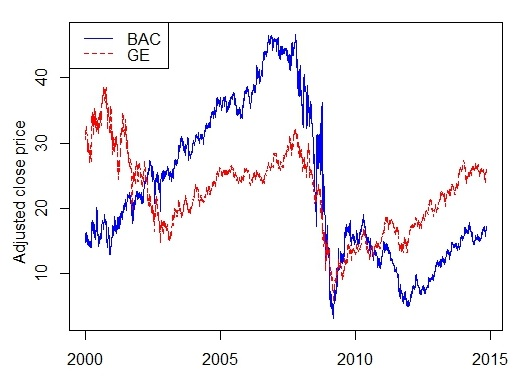
\includegraphics[scale=0.7]{BACGE}
					\caption{Time plot of daily stock returns (in US dollar) of BAC and GE, from January 2000 to November 2014. The blue line represents 
					Bank of America, and the dashed red line represents General Electric Inc.}
					\label{fig:bacge}
				\end{center}
			\end{figure}

			%#########################################################################################################################				
			\subsubsection{Data Properties}
			%#########################################################################################################################
				
			In Figure~\ref{fig:bac} and~\ref{fig:histbac} I see BAC's average price is $22.943$ USD, and it fluctuates in range of $3.053$ USD and 
			$46.582$ USD. The average log return is $0.0000245$, and the log returns fluctuates in range of $-0.3420578$ and $0.3020965$.

			\begin{figure}
				\begin{center}
					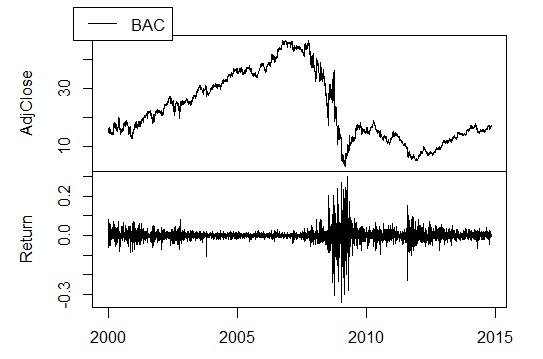
\includegraphics[scale=0.6]{BAC}
					\caption{Upper sub-panel is the time plot of daily stock returns (in US dollar) of GE from January 2000 to November 2014. Lower 
					sub-panel represents the respective log stock returns.}  
					\label{fig:bac}
				\end{center}
			\end{figure}

			In Figure~\ref{fig:ge} and~\ref{fig:histge} I see GE's average price is $21.855$ USD, and it fluctuates in range of $5.479$ USD and $37.866$ 
			USD. The average log return is $-0.0000584 $, and in between $-0.1368414$ and $0.1798441$. 
		
			\begin{figure}
				\begin{center}
					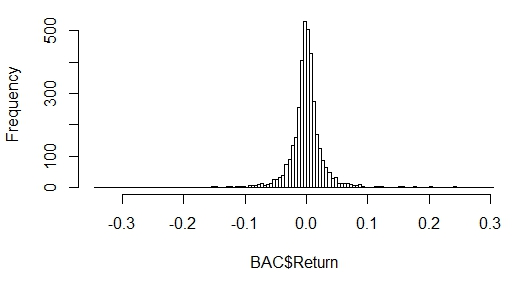
\includegraphics[scale=0.6]{HistBAC.PNG}
					\caption{Histogram of the log returns for Bank of America.}
					\label{fig:histbac}
				\end{center}
			\end{figure}
		 
			\begin{figure}
				\begin{center}
					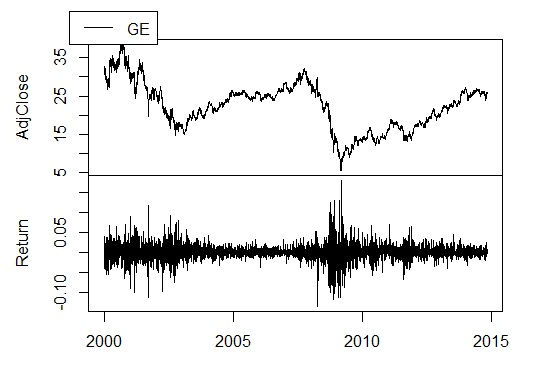
\includegraphics[scale=0.6]{GE.JPG}
					\caption{Upper sub-panel is the time plot of daily stock returns (in US dollar) of GE from January 2000 to November 2014. Lower 
					sub-panel represents the respective log stock returns.}
					\label{fig:ge}
				\end{center}	
			\end{figure}

			\begin{figure}
				\begin{center}
					\includegraphics[scale=0.6]{HistGE.JPG}
					\caption{Histogram of the log returns for General Electric.}
					\label{fig:histge}
				\end{center}
			\end{figure}
			
			A normal quantile-quantile (henceforth, Q-Q) plot shows a relation of residuals against fitted values. The Q-Q plots, for both stocks, reveals 
			some pretty heavy tails. This indicates that that the data frames that I am looking at, definitely are not normally distributed. Luckily for 
			us, this is actually desirable in our case, because ARCH(m) processes do have heavier tails than a normal distribution, cf.~\ref{subsec:arch}. 
			I proceed with my analysis. 
	
			\begin{figure}[H]
				\begin{center}
					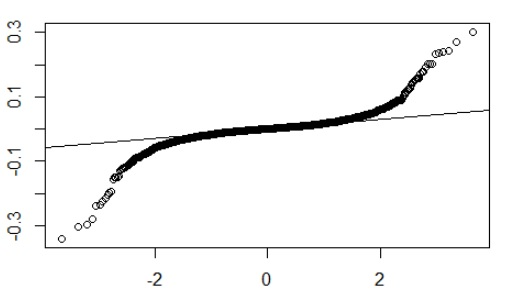
\includegraphics[scale=0.6]{bacqqplot.JPG}
					\caption{The Normal Q-Q plot for BAC.}
					\label{fig:bacqqplot}
				\end{center}
			\end{figure}
		 
			\begin{figure}[H]
				\begin{center}
					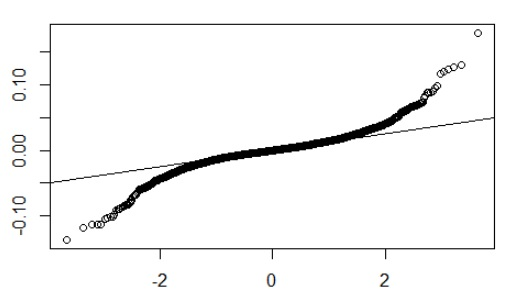
\includegraphics[scale=0.6]{geqqplot.JPG}
					\caption{The Normal Q-Q plot for GE.}
					\label{fig:geqqplot}
				\end{center}
			\end{figure}

			
			%#########################################################################################################################				
			\subsubsection{Identifying ARCH Process}
			%#########################################################################################################################				
        
        	The identification (or testing) of ARCH(m) process is a two-step procedure. The first step, is to verify if the time series has no (or, in some 
        	minor order) serial correlation between its past values. The second step, is to confirm that these series, actually have conditional
        	heteroscedasticity in one of its sub-populations.   
    
     		In Figure~\ref{subfig:bacacf1} and Figure~\ref{subfig:geacf1}, that both series have no serial correlations (i.e., the log returns are within 
     		the two standard-error lines, on the magic $5\%$ significance level).

			\begin{figure}[H]
				\centering
				\begin{subfigure}[b]{0.95\textwidth}
					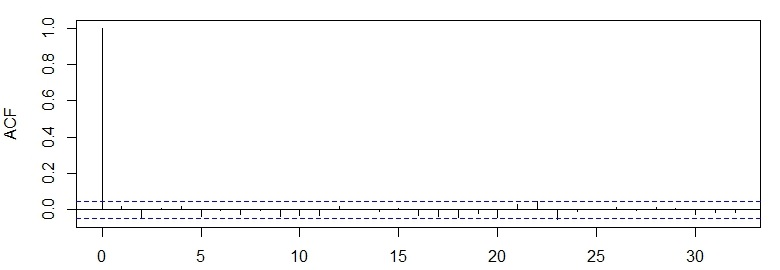
\includegraphics[width=1\linewidth]{BACACF}
					\caption{The sample autocorrelation function of the log return series for BAC}
					\label{subfig:bacacf1} 
				\end{subfigure}
				\begin{subfigure}[b]{0.95\textwidth}
					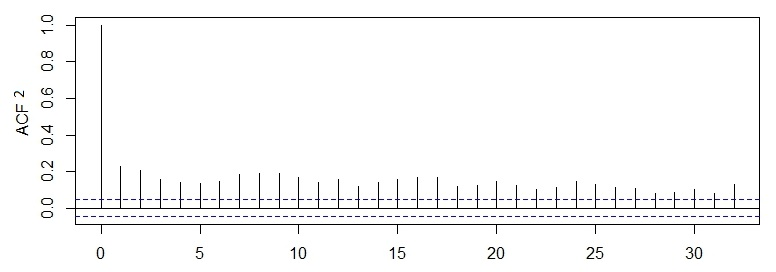
\includegraphics[width=1\linewidth]{BACACF2}
					\caption{The sample ACF of the squared log returns series for BAC}
					\label{subfig:bacacf2}
				\end{subfigure}
				\caption[numsol]{The sample ACF of two various functions of daily log stock returns for Bank of America, where the sample period is 
				from January 2000 to April 2014.}
				\end{figure}
			
			In Figure~\ref{subfig:bacacf2} and Figure~\ref{subfig:geacf2}, I see that there is somewhat exponential decay pattern, for both 
			series. Although, the patterns are not like a perfect textbook example of an exponential decay pattern, I choose to proceed with testing our
			null hypotheses.

			\begin{figure}[H]
				\centering
				\begin{subfigure}[b]{0.95\textwidth}
				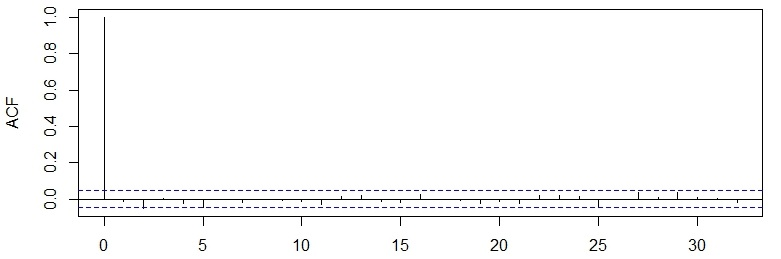
\includegraphics[width=1\linewidth]{GEACF}
					\caption{The sample autocorrelation function of the return series for GE}
					\label{subfig:geacf1} 
				\end{subfigure}
				\begin{subfigure}[b]{0.95\textwidth}
					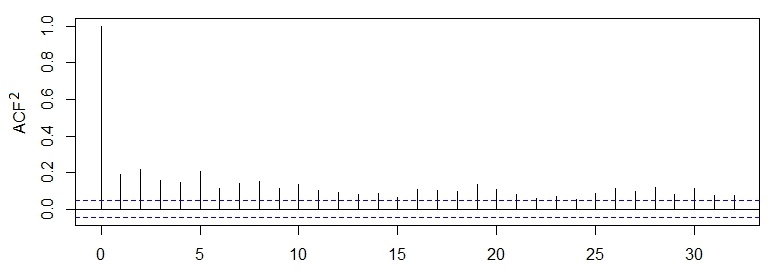
\includegraphics[width=1\linewidth]{GEACF2}
					\caption{The sample ACF of the squared log returns series for GE}
					\label{subfig:geacf2}
				\end{subfigure}
				\caption[numsol1]{The sample ACF of two various functions of daily log stock returns for General Electric, where the sample period is 
				from January 2000 to April 2014.}
				\end{figure}


			%#########################################################################################################################						
			\subsubsection{Testing for Autocorrelation}
			%#########################################################################################################################
			
			The Ljung-Box $Q(m)$ statistic for BAC log returns is $Q(8) = 9.2565$ with p-value $0.3211$. The test is not significant (on a $5\%$ level), 
			and I cannot reject our hypothesis that there is no serial correlation in the time series. The Ljung-Box $Q(m)$ statistic for GE log returns 
			is $Q(8) = 10.9671$ with p-value $0.2036$. The tests is not significant, and I cannot reject our hypothesis that there is no serial 
			correlation in the time series. Since, the series do not have any significant serial correlations, I continue to testing for ARCH Effect.		
			
			
			%#########################################################################################################################			
			\subsubsection{Testing for ARCH Effect}
			%#########################################################################################################################
		  
			Once again, I use usual Ljung-Box $Q(m)$ statistics, but this time to the squared time series $r^2_t$. The Ljung-Box $Q(m)$ statistic for BAC 
			has p-value $< 2.2e-16$. The test is significant, and I conclude that BAC has some conditional heteroscedasticity. The Ljung-Box $Q(m)$ 
			statistic for GE has p-value $< 2.2e-16$. I find this test, also to be significant, and I conclude that GE has some conditional 
			heteroscedasticity effect.  \vspace{0.3cm}
			
			Okay, so now that I have the relevant dataset, I want to talk more about Bayesian statistics.  





	%##############################################################################################################################################
	%##############################################################################################################################################	
	%##############################################################################################################################################
	\section{Bayesian Statistics} \label{sec:bayesianstatistics}
	%##############################################################################################################################################
	%##############################################################################################################################################
	%##############################################################################################################################################


		%#########################################################################################################################
		\subsection{Introduction}						
		%#########################################################################################################################

		Reverend Thomas Bayes (1701 - 7 April 1761) was an English statistician, philosopher and Presbyterian minister. Bayes by strong mathematical 
		reasoning proved the latter famous Bayes' theorem. His work was posthumously published in 1763 by his friend Sir Richard Price. 
		Some time after, independently of the publication, a French mathematician and astronomer Pierre-Simon Laplace generalized Bayes' theorem 
		(but mostly in words). Price and Laplace have met in Paris, and talked together, and Laplace did recognized that Bayes was the first who
		mathematically have proved the theorem. Laplace was the pioneer in his vision and have popularized Bayesian probability even 
		further~\footnote{\url{http://en.wikipedia.org/wiki/ Thomas_Bayes}}. Many years later, or more precisely in the early 1990s, Bayesian inference 
		reached mainstream statistics. 
			
		Bayesian statistics is an alternative approach to the classical frequentist approach, that most students have to learn in both graduate and 
		undergraduate statistics courses. The main difference, is in the philosophical view and aspects of Universe and its 
		mutual interconnectivity. Thus, the Bayesian statisticians believe that a world they choose to model, has dependent probabilities. Such that, these 
		conditional probabilities, somehow and in some way, always conditioned on something. This assumption makes it possible, to update a subjective 
		knowledge and experience about a phenomenon, by recalculating personal a priori probability density function. 
	
		The general nature of a Bayesian framework is a systematic updating statistical technique of various conditional probabilities. I think that the
		one of the most fascinating thing about this theorem is that tedious repetitive calculations, that in most cases very difficult and if not 
		impossible computational tasks, now can be (to a certain degree) easily calculated with use of a modern laptop computer. I believe that Bayes 
		statistics and use of it, will only become more and more popular in the future, with further growth in modern computer processing power.
	
		To gain a better understanding and more profound insight into Bayesian statistics, the interested reader might want to consult, for 
		example~\citep[chap. 2.1]{lee} or \citep[pp. 241-243]{brandimarte}.


		%#########################################################################################################################
		\subsection{Bayes' Theorem}						
		%#########################################################################################################################

		\textit{Bayes' theorem} (also known as Bayes' rule, Bayes' law, or Bayes' formula) is one of basic logical reasoning pillars in both probability 
		and statistics. Alternatively, formulated and often referred to as a~\textit{theorem on the probability of causes}. Although Bayes' theorem easily 
		can be deduced with a pencil on a piece of paper~\citep[pp.~7-17]{schaum}, I do believe that it very well may take several years to truly 
		understand the theorem and various applications of it. 
		
		Suppose there is a sample space $S$ with only two but mutually exclusive events, i.e. $A$ and $B$ such that $P(B) > 0$. Furthermore, let 
		$P(A\text{ }|\text{ }B)$ denote respective conditional probability of $A$, given that $B$ is known and has occurred. Since I can observe a value 
		of $A$ when event occurs, I can update the original $S_t$ with a new sample space $S_{t+1}$. Hence, I can write 
		$P(A\text{ }|\text{ }B) = P(A \cap B)/P(B) \Leftrightarrow P(A \cap B) = P(B) P(A\text{ }|\text{ }B)$. Due to symmetry, I can write same 
		differently $P(B\text{ }|\text{ }A) = P(A \cap B)/P(A) \Leftrightarrow P(A \cap B) = P(A) P(B\text{ }|\text{ }A)$. Because of the equality I 
		can write $P(A \cap B) = P(A) P(B\text{ }|\text{ }A) = P(B) P(A\text{ }|\text{ }B)$. Thus by dividing with $P(B)$ I can obtain Bayesian theorem  

		\begin{eqnarray*}
			P(B \text{ }|\text{ } A) = \frac{P(A) P(A\text{ }|\text{ }B)}{P(B)}.
		\end{eqnarray*}
		
		\noindent The denominator $P(B)$ can be calculated (mostly in simple cases) by using the law of total probability. In practise, in some financial 
		applications, the event $B$ is a result in one of mutually exclusive events $A_1, A_2,\ldots, A_T$. That is, in a discrete case can be written as

		\begin{eqnarray*}
			P(B^\ast) &=& P(A_1)P(B \text{ } | \text{ }A_1) + \cdots + P(A_T)P(B\text{ } | \text{ }A_T) \\
	     			  &=& \sum_{t=1}^T{P(A_t)P(B\text{ }|\text{ }A_t)}  	
		\end{eqnarray*}
		
		\noindent It is worth noting that, in most simple cases I can integrate $P(B^\ast)$ analytically, but in more complex cases (i.e., 
		multidimensional state spaces) I can only simulate an approximative solution by using e.g. Markov Chain Monte Carlo techniques. 
	
		%#########################################################################################################################
		\subsection{Posterior is prop to prior times likelihood}
		%#########################################################################################################################

		Consider the problem where a stock analyst observes daily returns for various publicly traded stocks. Sooner or later, the stock analyst may 
		realize that some of the stocks have clear characteristic repetitive cyclical patterns (due to e.g. a seasonality within a seasonality). Based on 
		relevant data, solid mathematical apparatus and a good portion of scientific epistemological intuition, the stock analyst will eventually generate 
		own trading ideas and investment strategies. Such that, gradually through time, an investment philosophy will be born, evolved and various trading 
		rules defined and written. 
	
		Now, without further ado, let the so-called trading rules, mathematically very well fit into the following pattern. Furthermore, assume that these 
		trading rules can be represented with a random vector of some exogenous variables. I can denote this latent vector $\theta$ of unknowns as 

		\begin{eqnarray*}
			\theta = (\theta_1, \theta_2, \ldots, \theta_k), 		
		\end{eqnarray*}	

		\noindent where $k \geq 1$ is the number of respective parameters. In other words, $\theta$ represents quantity-values of unknown implicit 
		parameters, (which usually either integers and/or real numbers), that I wish to estimate, because these parameters characterize a distribution of 
		interest for the respective stock returns.  This is the main reason why, I am so interested in estimating $\theta$, as it characterizes pdf for a 
		random sample of $X$ of returns. Suppose, that I can write the vector $X$ of random variables as a sequence 
		
		\begin{eqnarray*}
			X=(X_1, X_2,\ldots, X_T),		
		\end{eqnarray*}
		
		\noindent where $T \geq 1$ is the total number of observations in a data set series. In other words, the respective density function of a stock 
		quotes is dependent on $\theta_k$ latent parameters. 

			%###########################################################################################################
			\subsubsection{Prior Beliefs}
			%###########################################################################################################
	
			Assume that the analyst, in advance, makes various observations on a stock market, before even s/he have collected any evidence and relevant 
			data. I can express this subjective a priori knowledge as pdf
			
			\begin{eqnarray*}
				p(\theta) = p(\theta_1, \theta_2, \ldots, \theta_k),		
			\end{eqnarray*}
			
			\noindent which is also called a priori distribution, that expresses the analyst's beliefs about parameters in the $p(\theta)$ of $\theta$.
	
			Now, here it is worth noting that the more empirical data becomes available to the stock analyst, the less weigh her/his prior beliefs. But 
			then again, as the Oracle of Omaha Warren Buffett says: "We are all created equal, but we do not all have an equal opportunity." In other 
			words, in context of this thesis, in real life "big data" costs money and not every stock analyst can afford it. 				

			
			%###########################################################################################################
			\subsubsection{Likelihood Function}
			%###########################################################################################################
   
			The likelihood function $L(\theta \text{ } | \text{ }X)$ measures how likely is an observation $i$ in $X =\{r_i\}_{i=1}^T$ for a given value 
			of parameter $\theta$. Hence, by using likelihood function, I can express the conditional density function $f(X\text{ }|\text{ }\theta)$ as
			
			\begin{eqnarray*}
				L(\theta \text{ } | \text{ }X) &=& f(X\text{ }|\text{ }\theta) =  f(X\text{ }|\text{ }\theta_1, \theta_2,\ldots, \theta_k) \\
				&=& f(r_1, r_2,\ldots, r_T \text{ }|\text{ } \theta_1, \theta_2,\ldots,\theta_k) \\
				&=& f(r_1 \text{ }|\text{ } \theta) f(r_2 \text{ }|\text{ } \theta)\cdots f(r_T \text{ }|\text{ } \theta),
			\end{eqnarray*}	 
	
			\noindent where $X$ is a sequence of $T$ observations/realizations with known values, that are conditionally on $\theta$. 

			
			%###########################################################################################################
			\subsubsection{Posterior Distribution}
			%###########################################################################################################

	
			I am interested in a distribution of unknown $\theta$ given observed $\{r_i\}_{i=1}^T$. I estimate a distribution of $\{r_i\}_{i=1}^T$ for 				known fixed $\theta$. Hence, I want to invert a conditioning on $\theta$ to conditioning on $\{r_i\}_{i=1}^T$. Hence, I use Bayes' theorem 
			and merge the respective likelihood and prior beliefs, such that I get 
		
			\begin{eqnarray*}
				f(\theta \text{ } | \text{ }r_1, r_2,\ldots, r_T) = \frac{1}{Z}f(\text{ }r_1, r_2,\ldots, r_T \text{ } | \text{ } \theta)p(\theta),
			\end{eqnarray*}	 
			
			\noindent where $Z$ is  a normalizing constant. By applying the total probability theorem, for given $f(X\text{ }|\text{ }\theta)$ 
			distribution and $p(\theta)$ distribution of prior beliefs, I can find a normalizing constant $Z$, as the marginal density for 
			$X_1,\ldots X_T$

			\begin{eqnarray*}
				Z = \int_\Theta f(\{r_t\}_{t=1}^T \text{ }|\text{ }\theta)p(\theta)d(\theta),
			\end{eqnarray*}	 
	 		
	 		\noindent where I integrate over area where $\theta$ is well defined in domain $\Theta$. Since $\theta$ is independent of $\theta$, it 
	 		does not change the shape of the distribution, and I can disregard from it. For more convenient notation I can write 
	 		
			\begin{eqnarray*}
				p(\theta \text{ } |\text{ } D) &\propto& p(D \text{ } |\text{ } \theta )p(\theta),
			\end{eqnarray*}
			
			\noindent where the $p(D \text{ } |\text{ } \theta )$ is the prior probability distribution $p(\theta)$ of $\theta$. This is just an 
			epistemological intuition that a scientist decision/inference biased to believe about the prior beliefs. For more memorable version of the 
			theorem I can write
			
			\begin{eqnarray*}
				\text{posterior} \propto \text{prior} \times \text{likelihood},
			\end{eqnarray*}	 
			
			\noindent in other words says that I merge likelihood with prior knowledge of observed data.
				
		
		%#########################################################################################################################
		\subsection{The Proposal Density}
		%#########################################################################################################################
	
	
		FUBINI START \\	
		Imagine that we can thi
		
		To better understand the proposal density function, let us take a closer look at the following illustrative example. Suppose, that there exists an 
		explicit 
		mathematical solution, that logically can be deduced with an old-school pen and pencil on some pieces of papers method. That is to find the
		solution the group of ARCH(1) stochastic processes parameters. Thus these two appropriate modelling choices for the\textit{a priori distribution}
		could for example look like that. 	
	
		FUBINI SLUT \\	
	
			%###########################################################################################################
			\subsubsection{Our Choice of Prior Distribution}
			%###########################################################################################################
	
			In the first case, I can write our a priori distribution, as the product of two independent exponential distributions for both 
			$\alpha$-parameters
			
			\begin{eqnarray} \label{eq:prior}
				p(\alpha_0, \alpha_1) &=& \frac{1}{\beta_0}\exp{(-\frac{\alpha_0}{\beta_0})}\frac{1}{\beta_1} \exp{(-\frac{\alpha_1}{\beta_1})}, \text{ } 
				\alpha_0, \alpha_1, \beta_0, \beta_1 > 0
			\end{eqnarray}
	
			where $\alpha_0$ and $\alpha_1$ are the two unknown parameters, and $\beta_0$ and $\beta_1$ are their respective means.

			I choose to use this a priori distribution in our numerical implementation of ARCH(1) model.
	
			
			%###########################################################################################################
			\subsubsection{Alternative Choice of Our Prior Distribution}
			%###########################################################################################################
	
			In the second case, I can write an alternative a priori distribution, where I can choose to believe the ARCH(1) process has a variance. 
			In that particular case, I know that $\alpha_1 < 1$. That is, the alternative a priori distribution must satisfy $\alpha_1 > 0$ and 
			$\alpha_1 < 1$. Hence, the a priori distribution is a product of an exponential distribution for $\alpha_0$, and uniform distribution 
			$U \sim \left[0, 1\right]$ for $\alpha_1$, is given by 
			
			\begin{eqnarray*}
				p(\alpha_0, \alpha_1) &=& \frac{1}{\beta_0}\exp{(-\frac{\alpha_0}{\beta_0})}\cdot 1, \text{ where } \alpha_0  \text{ and } \beta_0 > 0.
			\end{eqnarray*}
	
			It can be a possibility to use this the alternative a priori distribution in the numerical implementation of ARCH(1) model.


		%#########################################################################################################################
		\subsection{Our Posterior Distribution}
		%#########################################################################################################################
	
		% I now turn to our posterior distribution\ldots given the "data" $r$ vector of excessive returns.
		Okay, perfect\ldots progress!.. Finally, I figure out how to I can derive our posterior distribution. By rearranging 
		equations~\ref{eq:lik} and ~\ref{eq:prior}
		(where the unknown parameters $\alpha$ are conditioned on a stock return in a times series), I get the following result 
	
		\begin{eqnarray*}
			\pi\left(\alpha_0, \alpha_1 \text{ }| \text{ } r \right) = \prod_{t=2}^T{\frac{1}{\sigma_t}\exp{\left(-\frac{r^2_t}{2\sigma_t^2} \right)}}					\frac{1}{\beta_0}\exp{\left( -\frac{\alpha_0}{\beta_0}\right)}\frac{1}{\beta_1}\exp{\left(-\frac{\alpha_1}{\beta_1}\right)}. 
		\end{eqnarray*}	 	
	
		The respective \textit{log-likelihood (lik)} function, where I am disregarding from a (probably unknown) normalizing constant. Our lik is

		\begin{eqnarray} \label{eq:posteriori}
			\log{\left( \pi\left(\alpha_0, \alpha_1 \text{ } | \text{ } r \right)\right)} &=& \sum_{t=2}^{T}{\log{\frac{1}{\sigma_t}}
			\exp{\left(-\frac{r^2_t}{2\sigma_t^2} \right)}} + \log{\left(\frac{1}{\beta_0} 
			\exp{\left(-\frac{\alpha_0}{\beta_0} \right)} \right)}\nonumber \\
			&&+ \log{\left(\frac{1}{\beta_1} \exp{\left(-\frac{\alpha_1}{\beta_1} \right)} \right)} \nonumber \\
			&=& \sum_{t=2}^{T}{\left( \log{\frac{1}{\sigma_t} + \frac{r_t^2}{2\sigma_t^2}} \right)} + \log{\left(\frac{1}{\beta_0}\right)} 
			- \frac{\alpha_0}{\beta_0} \nonumber \\
			&&+ \log{\left(\frac{1}{\beta_1} \right)} - \frac{\alpha_1}{\beta_1} \nonumber \\
			&=& \sum_{t=2}^{T}{\left( \log{\frac{1}{\sigma_t} + \frac{r_t^2}{2\sigma_t^2}} \right)} - \frac{\alpha_0}{\beta_0} - 
			\frac{\alpha_1}{\beta_1}.
		\end{eqnarray}	 	
	
		\noindent After, I have been looking at our posterior for quite some time, I am pretty much convinced that our deduced distribution has no 
		explicit solution (at least to us known). 
								
			%###########################################################################################################
			\subsubsection{Full Conditionals}
			%###########################################################################################################	
	
			In addition to the posterior distribution, I take a brief look at two full conditionals. Such that, the first full conditional 
			for $\pi_{\alpha_0}$, that is conditioned on $\alpha_1$ and $r$ is represented by
				
			\begin{equation*}
				\pi_{\alpha_0} \left( \alpha_0 \text{ }|\text{ } \alpha_1 , r \right) \propto \prod_{t=2}^T{\frac{1}{\sigma_t}\exp{\left(-\frac{r^2_t}
				{2\sigma_t^2} \right)}}\frac{1}{\beta_0}\exp{\left( -\frac{\alpha_0}{\beta_0}\right)},
			\end{equation*}	 
			
			\noindent whereas, the second full conditional for $\pi_{\alpha_1}$that is conditioned on $\alpha_0$ and $r$  is given by

			\begin{equation*}
				\pi_{\alpha_1} \left( \alpha_1 \text{ }|\text{ } \alpha_0 , r \right) \propto \prod_{t=2}^T{\frac{1}{\sigma_t}\exp{\left(-\frac{r^2_t}
				{2\sigma_t^2} \right)}}\frac{1}{\beta_1}\exp{\left( -\frac{\alpha_1}{\beta_1}\right)}.
			\end{equation*}	 
			
			
			\noindent Similarly, as with our posterior distribution, I simply cannot recognize the full conditionals. Intuitively, I am now convinced 
			that neither our posterior or the full conditionals, can be solved explicitly. Unfortunately for us, it looks like I have to get our hands 
			dirty, and do some statistical computations and numerical programming. Alas, first I have to learn more about Markov Chain Monte Carlo 
			methodology. I begin our study with Markov chain theory.








	%##############################################################################################################################################			
	%##############################################################################################################################################
	%##############################################################################################################################################

	\section{Markov Chain Theory} 

	%##############################################################################################################################################			
	%##############################################################################################################################################
	%##############################################################################################################################################

		%###########################################################################################################
		\subsection{Introduction} 
		%###########################################################################################################


		Andrey Andreyevich Markov (1856 - 1922) was a Russian and then later a Soviet mathematician. He was a student of another prominent Russian 
		mathematician, namely Pafnuty Lvovich Chebyshev (1821 - 1894)~\footnote{\url{https://en.wikipedia.org/wiki/Andrey_Markov}}, who is famous for his 
		mathematical contribution in the fields of probability, statistics, mechanics, and number  
		theory~\footnote{\url{https://en.wikipedia.org/wiki/Pafnuty_Chebyshev}}. Andrey Andreyevich is best known for his research in Markov Chain theory, 			which is a field in stochastic processes. In older works Markov was spelled as Markoff, and one of the oldest sources that I could verify was 
		found in~\citep[p.~341]{ulam}. 
		Andrey Andreyevich was inspired by a novel in verse "Eugene Onegin" that was written by one of he greatest Russian poet, author and writer 
		Alexander Sergeyevich Pushkin (1799 - 1837)~\footnote{\url{https://en.wikipedia.org/wiki/Alexander_Pushkin}}. The reader can find various excellent 
		partial translations of Pushkin’s poem can be found at Peter M Lee's 
		homepage~\footnote{\url{http://www-users.york.ac.uk/~pml1/onegin/partial.htm}}. Though, I have not been able to find the original work of Andrey 
		Andreyevich, such that, I could attempt to recreate his original thought processing, although that could be interesting to do that. Nevertheless, I 
		guess that I have been lucky two meet the primary school teachers~\footnote{\textit{Nadezhda Nikolajevna Vasilieva} and \textit{Nina 
		Gevnadivna Potapova} in Russian Litterature and Language in the primary schools nr. 3 and nr. 5, Sibiria, Republic Tuva} that were especially found 
		of Russian poetry, that is, as a pupil I had to recite of by heart various parts of Pushkin, back in old school days. I think, or still, as 
		Bayesians qualitatively guessing, that Andrey Andreyevich began to look at some different sequences (e.g. vocal combinations) of consonants and 
		vocals. Then after have been looking in vain at different combination of letters and these letters in words 
		combination, at some point he must have zoomed out of the sequence of words, and looked at the whole particular subsections of the poem. The poetry 
		of Alexander Sergeyevich, in my humble opinion, is a close  to some-kind of combination of hip hop rhyming and written poetry of an English poet, 
		playwright and actor William Shakespeare. To be honest with the reader, it is impossible to recite whole poem, especially if you try to remember 
		all words, key words, pictures, images, etc\ldots. But by remembering phonetics and particular rhythm of subsections, that have some kind of 
		different waves formation, one can surely recite the poem of by heart for hours.  So, and I am still guessing, Andrey Andreyevich must have 
		realized that rhythm of next subsection (i.e., future) was independent of all other subsections (i.e., past) except from the present subsection 
		(i.e., present), which is by the way is one of the key notions of a Markov chain. Now, maybe it is not that surprising too see that (hidden) Markov 
		chains are heavily used in speech recognition and digital signal processing as well. 
		
		The reader can find more interesting details with rigorous mathematical examples, derivations and proofs, 
		inter alia~\cite{chib},~\cite{chib1}[pp. 3576--3579],~\cite{gamerman}[pp. 93-116], ~\citep[p. 246]{lee}, and~\cite{monahan}[pp. 375-400]. 

	
		%###########################################################################################################
		\subsection{Finite Markov Chains} 
		%###########################################################################################################

		
		Assume that I have a $d$-dimensional continuous state space, where a transition kernel 

		\begin{equation*}
			Pr(x, A) = 
		\end{equation*}
	
		a conditional distribution function is represented with 

		Fubini et de Finetti,\ldots, logically speaking, thoughts in process 
	
		I assume that there exists the unique stationary distribution (the limiting distribution) $\pi$, such that the initial distribution 
		(i.e. initial state of a system) a chain $\pi^{\left(n\right)}$  

		~\cite{lawler}[pp. ]


			%#########################################################################################################################
			\subsubsection{Notation}
			%#########################################################################################################################
			
			To keep consistent notation as clear as possible, I 


			%#########################################################################################################################
			\subsubsection{Stationary Distribution}
			%#########################################################################################################################


			%#########################################################################################################################
			\subsubsection{Reversibility of Chains}
			%#########################################################################################################################



			
		%############################################################################################################
		\subsection{Continuous State Space} 
		%############################################################################################################

		The continuous time processes case
		
			%#########################################################################################################################
%			\subsubsection{Transition kernels}
			%#########################################################################################################################

			%#########################################################################################################################
			\subsubsection{Fubini Fuck}
			%#########################################################################################################################

			%#########################################################################################################################
			\subsubsection{Fubini Head}
			%#########################################################################################################################






			




	%##############################################################################################################################################			
	%##############################################################################################################################################
	%##############################################################################################################################################
	\section{Markov Chain Monte Carlo}
	%##############################################################################################################################################	
	%##############################################################################################################################################
	%##############################################################################################################################################


		%###########################################################################################################
		\subsection{The Short Motivation to MCMC} 
		%###########################################################################################################

		In statistics, or maybe more precisely in statistical modelling, Markov Chain Monte Carlo (henceforth, MCMC) is a very big algorithmic family of 			various mathematical schemes, computational methods and numerical implementation techniques. 
		
		I must admit at once, that there is going on a gigantic research in this vast MCMC field. There are myriads of flourishing academic 
		literature. Such that there are many excellent examples of various pseudo - and implemented algorithms. Various software tools, scientific 
		programming and higher order probabilistic programming languages out there~\footnote{e.g., Anglican, BUGS, Church, Fortran, GAUSS, JAGS, 
		Mathematica, Matlab, OpenBUGS, Python, R, Stan, Venture, WinBUGS, \ldots}, that are now available to any scientist. 
		
		I must also admit that I did only a very short, but I must say at the same time quite intense, introduction study to MCMC subject. Gradually 
		it sort of became obvious to us how powerful MCMC techniques are, though I am still in the learning process mode. Nevertheless, as I 	
		understand the secret of these MCMC techniques is not only in the rigorous mathematical notation. But also, it is as much in various hands-on 
		numerical challenges of being able to implement on available modern computational facilities. 
		
		I think, and I must admit that from now on only subjectively, that MCMC methodology in modern statistics (also in e.g., economics, 
		econometrics, image analysis, machine learning, physics, robotics, social science, etc\ldots), is a powerful all-round computational mechanisms 
		that definitely can be used for estimation of a model's latent parameters. Not only that, I also think that MCMC can be used to do various 
		strategic Hedge Fund's investments strategies on a volatility's fluctuations, for various publicly traded stocks and financial instruments. 
		Although, to be honest with the reader, I do not really know how to do it, yet. But I have an idea, how it should be done. 

		I believe, and from now on only subjectively, that I finally became completely Bayesians in our philosophical and statistical points of view. 
		Thus, I now see our numerical world with all available information to us, can and should be modelled with MCMC (even if it 
		is computationally costly and time consuming), mainly because I am believing in future increasing computational power. Thus, in other words, if 
		MCMC techniques wisely used and cleverly implemented, it can certainly be the universal magic hack for finding "exact" solutions to (almost) any 
		physical phenomena (that by the way, cannot be solved with traditional pure mathematics in various branches of nature science and wide variety of 
		situations.  
		
		So maybe after all it was not that bad idea to get our hands fully dirty!.. Hence, I with our heads first, jump into Ocean dé MCMC. 

		
		%###########################################################################################################
		\subsection{The Not So Short Introduction to MCMC} 
		%###########################################################################################################

		In this subsection, I will try to give a brief introduction, somewhat short overview and historical background on MCMC. Our subjective 
		discussion is mainly based on~\cite{robert}, where it is interesting to read about the inception, revolution and post-revolution era of MCMC and 
		its tremendous impact on modern computational statistics. The reader can skip this subsection without loss of continuity.
		
		The very first rudimentary version of \textit{Monte Carlo} (henceforth, MC) methods, actually was discovered in early 1930s by Italian physicist 
		Enrico Fermi. By the way, who also have invented the analogue device FERMIAC (or the Monte Carlo trolley), which could be used to model neutron 
		transportation in various types of nuclear systems\footnote{\url{http://en.wikipedia.org/wiki/FERMIAC}}. But since there was no modern electronic 
		computer machinery available at that time, alas he never got any recognition for his visionary work and profound insights in physics. 
		
		Nevertheless, it is common to say that the original methodology of MCMC computational techniques, initially was conceived in the secret Los 
		Alamos Scientific Laboratory, Los Alamos, New Mexico during the end of second World War and the beginning of the Cold War's arms race. Although, 
		MC and MCMC have been used in physics for quite some time, its impact first became influential in early 1990s. 
		
		The original idea to regular MC methods, can be traced all the way back to the late 1940s. The co-inventors of MC methods were a Polish and 
		later American mathematician Stanislaw Marcin Ulam, and John von Neumann a Hungarian and later American applied mathematician and physicist. 
		At some point, Ulam was looking at an intractable combinatorial computations of winning probability of "solitaire" card game. The main reason 
		was, that the combinatorics and probabilities of the game, were much similar in its structure to various problems in physical phenomena. And, 
		with this in mind, von Neumann enthusiastically adapted the idea, and used it on various calculations in thermonuclear and fission problems.
		At the same time in 1947, Ulam and Neumann have invented MCMC techniques, such as, Bayesian probability inversion modelling and accept-reject 
		techniques.   
		
		Soon after,~\citep{ulam} have published the very first paper about the Monte Carlo method, that presented the idea of using new statistical 
		approach to study integro-differential equations (which are known in the kinetic theory of gases, as the Boltzmann equations). I think that the 
		major breakthrough of the paper was the first mechanized computations of new numerical techniques for approximation of unobtainable "closed form" 
		solutions of various integrals. 
		
		So, in other words, in early 1950s, the same group of Los Alamos Laboratory scientists (and plus many prominent others) that were mainly 
		physicists, did some intensive research in mathematical physics. The research, by the way, also known as Top Secret "The Manhattan Project" 
		was sponsored by U.S. military. The main purpose was the development/creation of the first atomic bombs. Which are the Fruits of World War II. 
		During their amazing research process, they managed successfully to simulate MCMC computations, which were combined with the first computer 
		ENIAC\footnote{ENIAC stands for Electronic Numerical Integrator and Calculator, and was built with transistors in February 1946, after three 
		years of construction}, they were the first to succeed to generate computer simulations for various MC schemes. 
		 		
		Then, couple of years later, the discovered MC ideas were further studied and presented in the published paper by~\cite{metropolis}. Metropolis 
		et al. described the modified method of MC integration, where the efficiency was in the improvement of a random walk. It is reasonable to say 
		that the first MCMC method was the Metropolis algorithm (henceforth, MA). The generated numerical calculations were carried out on second Los 
		Alamos MANIAC computer~\footnote{MANIAC stands for Mathematical Analyzer, Numerical Integrator and Computer}. Believe it or not, it was the big 
		thing back then. Suddenly, it was numerically possible to use so-called fast machines and MCMC to obtain feasible experimental results to 
		statistical mechanical problems, that yet not have been possible to solve before for many-dimensional integrals. Metropolis et al. proved 
		ergodicity, which is sufficient condition for asymptotic convergence towards the stationary distribution of Markov chains. And proposed 
		integrating over a random sampling of points, such that respective stationary distribution of interest would be the Markov chain equilibrium of 
		the state of finite number $N$ of interacting individual molecules. By the way, the "Monte Carlo" name was suggested by Nicolas Metropolis, who 
		was both a physicist and mathematician.  

        Thereafter, or almost 20 years later the publications by~\citep{hastings} and his student~\citep{peskun} have further popularized MCMC 
        methodology. In a sense, they brought MCMC closer to various mainstream statisticians (i.e., social scientists, data scientists, economists, 
        etc\ldots). So, as mentioned above, MA (that was originally proposed by Metropolis et al.) is a sampling method (on a digital computer) that 
        requires the simulation of a Markov chain sequence with its respective specified stationary distribution. Now, that Hastings has introduced an 
        outline of such a generalized method of the sampling procedure, i.e., a recipe for how to construct and simulate such a Markov chain sequence. 
        Hastings (in his paper) likewise exposed relevant Markov chain theory and presented four examples. He has also discussed a challenging topic, 
        which namely is an assessment of the error of an estimation, produced by using Monte Carlo methods. Then short time after, P. H. Peskun in his 
        Biometrika paper did comparison of two sampling methods that were proposed by Metropolis et al. and Barker. Peskun thus has shown that in a 
        discrete setup, MA sampling method is asymptotically more precise than Barker's independent sampling. I would like to make one more comment 
        that~\citep{peskun81} further provided very intuitive and practical computational guidelines for choosing the transition matrix 
        $\underline{\underline{P}}=p_{ij}$, when using Monte Carlo methods in conjunction with Markov chain sampling.

		Then almost a decade later,~\citep{geman} have introduced their version of MCMC simulation technique, the alternative 
		approach~\textit{Gibbs Sampler} algorithm (henceforth, GS). The algorithm was named after an American physicist Josiah Willard Gibbs (1839-1903) 
		that developed the field of vector analysis and made contributions to crystallography and planetary orbits. Gibbs sampling is a fairly simple and 
		widely applicable MCMC algorithm. It is easy (although in the beginning can be little confusing) to see that GS is a special case of the 
		MH algorithm~\citep[pp.~542-543]{bishop}. Now, at this moment, I must note that Gibbs sampling and Metropolis-Hastings algorithm, originate from 
		two different sources, though the mathematical justification via Markov chains is same. So, Donald and Stuart 
		Geman~\footnote{The development of BUGS (Bayesian inference Using Gibbs Sampling) software, as early as 1991, was originally initiated by Geman 
		and Geman} have successfully presented  new ideas for a Bayesian restoration solution in image processing problems. They have also introduced the 
		generic description of Gibbs sampling, and proved that like MA, that GS produces a Markov chain with $\underline{\pi}$ as the equilibrium 
		distribution~\citep[p.~731]{geman}. 
		
		\citep{tanner} are like Geman and Geman are just one of earlier pioneers of GS. In the article, they have introduced an iterative method for 
		the calculation of posterior distributions. The data augmentation algorithm, with great advantage, can be used in solving maximum likelihood 
		problems.		 
		 			
		With all this in mind, as a result, Bayesian inference and MCMC methods have changed entire academic way of thinking and attacking different 
		phenomena and challenges in applied computational tasks. The numerical real-life problems, that could not be solved due to computational limits, 
		now became cracked open like eggs. I agree with~\citep{robert} that this can be one of paradigm shifts that originally defined by Thomas Kuhn. 			MCMC became a universal key or numerical wrench tool, you (i.e., the reader and the writer) can attack (almost) any numerical problem, even 
		shooting a house sparrow with a cannon. I therefore think that the demonstration of using various sequential mathematical computation steps, that 
		were made with help of the "first" artificial intelligence, laid ground not only to MCMC but also to modern numerical analysis.	

		The history of MCMC is short, but at the same time long. It is quite interesting history that is full of colourful details, just like one of the 
		paintings of a Dutch painter Vincent van Gogh (1853 - 1890). Thus, without a doubt, I will agree 100 percent with the reader that our~\textit{The 
		Not So Short Introduction to MCMC} and its respective chronological description of MCMC events, are insufficiently expressive. As I probably have 
		already mentioned above, there are and were many other prominent and influential research papers concerning MCMC techniques and computations. That 
		is, this is said, then this  should not be kept as a secret from the reader, that I do really want to read all available (to us) MCMC 
		nomenclature. And, yes-of-course, I would like to write more about MCMC history and different aspects of it, in the very near future. But, alas, 
		this exciting to-do-on-my-list-task-thing is beyond the scope, in the context of this thesis. 
		

		%################################################################################################################################
		\subsection{Thinking MCMC and Bayesian Inference} 
		%################################################################################################################################
		

		In section~\ref{sec:bayesianstatistics} I have introduced our subjective version of  Bayesian philosophy of science. I have also tried to expose 
		an introduction to a more detailed picture of an estimation method of various unknown parameters from some observed data series. In plain words, 	 	    I now can summarize the essence of the MCMC approach, in the following way. The observed posteriori statistical distribution of data observables
		is  actually equivalent to the merge-product (i.e., of iterative nature) of the (subjective nature) prior information and the likelihood of how 
		likely is a phenomenon to occur (on the basis of the current Bayesian belief(s)). So, in Bayesian framework I choose to regard the setup of 
		various unknown parameters (both discrete and/or continuous as random variables, and the respective probability of those random variables, as the 
		prior statistical distribution of interest. So, according to Bayes' theorem, the posterior density is a summary of our knowledge about the 
		parameters, that is merged (i.e., recursively) with a priori empirical evidence. 
		
		Now that I am well and heavy armed with the posterior distribution (and its continuously (i.e., recursively iterative iterations) updating 
		technique), I should be able to estimate the unknown parameters of interest. I can do that simply by finding their expected values. And, it is 
		worth noting that there is also possibility to find credible intervals (i.e., Bayesian confidence intervals), and do hypothesis testing of the 
		found parameters. But, there is always that little but in life and modelling. I do not know our normalizing constant in our posterior distribution. 
	    Our posterior is proportional to our prior multiplied with likelihood. And, even if I knew the normalizing constant, that is needless to say, the 
	    evaluation of multidimensional integrals is very difficult and certainly not easy to compute explicitly. However, there is this another possibility
	    that I have read so much about, in such relatively short time. The key idea is that I can sample from the posterior distribution. This way I
	    do not need to know the normalizing constant at all. Luckily for modellers like us, I utilize MCMC methods as sampling approaches to tackle the 
	    this normalizing constant that typically arises in analytically intractable problems (~\citep{brandimarte}[pp. 629-630, p. 647]).	

		Imagine (just like in the John Lennon's song) that you can imagine Bayesian Inference from a personal and epistemological rough knowledge point 
		view. The roughness or smoothness of zooming in and out process, can be controlled as with a matrix in multi dimensions. That is, the processed 
		knowledge based on information's data inputs becomes finer as more longer time Nature is being observed. Likewise originally, when looking 
		(gathering data) at an applied model (through finite period of time of usually equidistant steps) and its respective economic features, that 
		specified by various esoteric variables, a modeller can and should (gradually) be able to learn stochastically from her/his simulated data. Now, a 
		computational challenge of MCMC with interaction of modern digital computers, is the applied implementation of Bayesian inference. That is, as an 
		average business student e.g. like the writing writer faces great difficulty and challenge, that is not only in the pure mathematical notation, 
		economical insight and last but not least the numerical implementation of MCMC thinking with its practical Bayesian Inference in it.
				
		I prioritize our frugal time wisely and continue our focus on the numerical journey of MCMC algorithms!..
				
		%#########################################################################################################################
		\subsection{Metropolis-Hastings Algorithm}
		%#########################################################################################################################

		Why study algorithms, the reader may want to ask. Well, algorithms are all around us, and as economist and econometrist, the writing writer 
		can assure the reader that the algorithm are all around us, and are especially useful in financial and economic time series Bayesian data analysis
		\footnote{I understand definition of Bayesian data analysis as a numerical approximation to intractable explicit mathematical solution}.
		
		In order to be able to find mathematical sound solutions for various inference problems, I have to and must apply numerical principles of dynamic 
		programming.

the pronunciation and translation
			
		The Metropolis-Hastings Algorithm (henceforth, M-H)\ldots						
						
		%Fubini, litteratur referencen				
		For a more complete version of the M-H Algorithm see, for example work of,~\citep{chib},~\citep{gamerman}[chap. 6],~\cite{metropolis},
		~\citep{lee}[chap. 9.6] and~\citep{prochazka}[chap. 9.4.4].
			
		Note that via Markov chain theory the mathematical proofs for Metropolis-Hastings based algorithms and Gibbs samplers', mathematically 
		justified in the same way \citep[p.~1]{casella}.   
			
		The generic features of the Metropolis-Hastings algorithm
			
		An astonishing variety of versions of MH there are out there.			

		The art of programming 
						
			%#########################################################################################################################
			\subsubsection{Metropolis Algorithm}
			%#########################################################################################################################
			
			MA is a basic algorithm
			
			The MH algorithm is the same a Markov chain procedure 			
			

			
			The "Metropolis algorithm" produces a Markov chain 
			\begin{equation*}
				\left\{X\left(t\right), t=0,1,3\cdots \right\}				
			\end{equation*}						

			\noindent where the equilibrium of the chain is a stationary distribution $\pi$ (see \citep[p.731]{geman}. 
			
			Random walk Metropolis explores\ldots 

			
			% Draw; generate; repeat steps m-times; in this step 
			
			%%%%%%%%%%%%%%%%%%%%%%%%%%%%%%%%%%%%%%%%%%%%%%%%%%%%%%%%%%%%%%%%%%%%%%%%%%%%%%%%%%%%%%%%%%%%%%%%%%%%%%%%%%%%%%%%%%%%%%%%%%%%%%%%%%%%%%%%%%%%
			%Fubini, følgende skal omskrives:
			%The MC method for many-dimensional integrals consists simply of integrating over a random sampling of points instead of over a regular 
			%array of points (cf.~\citep[p. 1088]{metropolis}			
			%%%%%%%%%%%%%%%%%%%%%%%%%%%%%%%%%%%%%%%%%%%%%%%%%%%%%%%%%%%%%%%%%%%%%%%%%%%%%%%%%%%%%%%%%%%%%%%%%%%%%%%%%%%%%%%%%%%%%%%%%%%%%%%%%%%%%%%%%%%%
			
			\noindent The implementation of the algorithm should be straightforward, but in general, can be difficult and very challenging task to do. The 
			key idea that (business as usual) I want to cycle through the numerical procedure, by using for-loops and/or in some kind of combination with 
			while-loop.	
			
			%#########################################################################################################################	
			\subsubsection{Rejection Sampling Description}
			%#########################################################################################################################
	
			As far as I understand \citep[p.~267]{lee} says that, the \textit{acceptance-rejection sampling} is an important method, and a good place to 	
			start with Metropolis-Hastings algorithm. Although, this method does not make any use of Markov chain methods, it can be used directly in 					situations where a posterior distribution has an unknown normalising constant $Z$. In fact, assume that I have such a density
			$p(\theta)=f(\theta)/Z$ of interest, where $f(\theta)=x^{\alpha-1}(1-x)^{\beta-1}$ is given by a beta distribution. Now, assume also, that 
			there exist a respective \textit{candidate density} $h(\theta)$, such that I able to simulate samples from. Then, by simulating random 					variables $X$ from the $h(\theta)$, I can estimate a variate $\tilde{\theta}$ with respective $p(\theta)$. If one have no idea of what 					$h(\theta)$ should be, then a uniform distribution can be a good initial guess. Let us assume that $h(\theta) \sim U(0,1)$.  A more rigorous 				description of the acceptance-rejection sampling looks like this:
		
			\begin{enumerate}
				\item Generate a variate $y$ from $h(\theta)$.
				\item Generate a value $u \sim U(0,1)$.
				\item From step $1$ and step $2$, use generated values $u$ and $y$ to compare an equality $u\leq f(y)/kh(y)$, where $k>0$ is a known
				constant.
				\begin{enumerate}
					\item Then if the condition in step $3$ is true, then accept the variate $y$, assign it to vector $x$ of accepted values, and return 
					to step $1$ 
					\item Otherwise, return to step $1$.				
				\end{enumerate}	   		
			\end{enumerate}	   
	
			The algorithm can be implemented with a \textit{for-loop} with a \textit{while-loop} in it. The for-loop goes e.g. $N=1000$ times, and for 
			every iteration our while-loop calculates all 3 steps until the acceptance of $y$ is happened. When $y$ is accepted, jump out of while-loop, 
			increment for-loop with $1$ and begin while-loop again. 
	
			I can argue (both in the discrete and the continuous case) that the $\theta$ value in $N$ trials is on $Nh(\theta)$ 
			occasions. That is, the number of times that $Nf(\theta)$ retained is proportional to $f(\theta)$.

		
			%#########################################################################################################################
			\subsection{Metropolis-Hastings Algorithm}
			%#########################################################################################################################			
			
			Fubini\ldots, I can summarize the Metropolis-Hastings in the following algorithmic form: \\
	
			\noindent Fubini\ldots, for technically masterful explanations, see for example, Peter M Lee p. 270\\
			
			\noindent Fubini\ldots, something like that: Why do I want to use sampling, and what do I achieve from it? \\
			
			Metropolis-Hastings acceptance rule				
			
			an iterative algorithms that cycles through			
			
			%%%%%%%%%%%%%%%%%%%%%%%%%%%%%%%%%%%%%%%%%%%%%%%%%%%%%%%%%%%%%%%%%%%%%%%%%%%%%%%%%%%%%%%%%%%%%%%%%%%%%%%%%%%%%%%%%%%%%%%%%%%%%%%%%%%%%%%%%%%
			%FUBINI, følgende skal omskrives
			%Note that Metropolis et al. (1953) move one particle at a time, rather than moving all of them together, which makes the initial algorithm 
			%appear as a primitive kind of Gibbs sampler!.. (\citep[p.~3]{robert})
			%%%%%%%%%%%%%%%%%%%%%%%%%%%%%%%%%%%%%%%%%%%%%%%%%%%%%%%%%%%%%%%%%%%%%%%%%%%%%%%%%%%%%%%%%%%%%%%%%%%%%%%%%%%%%%%%%%%%%%%%%%%%%%%%%%%%%%%%%%%					
			% # acceptance prob is ratio, but bounded at 1
			% # M-H accept/reject step			
			% # store values

			for each time step $t$ I compute the acceptance test ratio corresponding $\frac{\text{TargetDist}}{PropDist}$
			a wide variety of situations

			the MH sampling method is an iterative Monte Carlo procedure
			
			, and it is important to realize that, the 
			
				%#########################################################################################################################
				\subsubsection{Definition and Properties}
				%#########################################################################################################################
			
				%%%%%%%%%%%%%%%%%%%%%%%%%%%%%%%%%%%%%%%%%%%%%%%%%%%%%%%%%%%%%%%%%%%%%%%%%%%%%%%%%%%%%%%%%%%%%%%%%%%%%%%%%%%%%%%%%%%%%%%%%%
				%Fubini, correct this line later
				% I perform an initial computation before collecting information in a burn-in phase (in other words, I run burn-in stage)
				% Discard the first 500 Draws as Burn-in
				%Fubini, correct this line later
				%%%%%%%%%%%%%%%%%%%%%%%%%%%%%%%%%%%%%%%%%%%%%%%%%%%%%%%%%%%%%%%%%%%%%%%%%%%%%%%%%%%%%%%%%%%%%%%%%%%%%%%%%%%%%%%%%%%%%%%%%%
			
				%Fubini - The acceptance probability is a ratio, but since I am in probability world, I bound the probability at 1 (if 
				%it have to make sense).
	
				The computation task is to find 			
			
	
		%###################11#######################################################################################################
		\subsection{Gibbs Sampling}
		%############################################################################################################################

		Okay, so why do I want to do sampling? 
		
		numerical integration is impossible			
			
		To see this, consider the 
		
		The computational approach 
		
		Big Fubini Stochastic thoughts processing in a matrix processes.
		
			%#########################################################################################################################
			\subsubsection{Introduction}
			%#########################################################################################################################
			
			Fubini, thoughts in process\ldots

			% Fubini, dette er kun et reference\ldots
			%the algorithm cycles m-step
			
			The reader who is interested in more theoretical details of GS's rigorous mathematical foundation, can for example 
			see~\citep[chap. 14]{brandimarte},~\cite{casella}, ~\citep{gamerman}[chap. 5],~\citep[p. 731]{geman},~\citep[chap. 9]{lee},
			~\citep{prochazka}[chap. 9.4.2], \citep{tanner} and~\citep[p. 388]{shumway}.			


			%############################################################################################################################
			\subsubsection{Definition and Properties}
			%############################################################################################################################


        The sampling strategy of a Gibbs algorithm, is an iterative scheme, where each respective component updated individually. To illustrate the 
        point, I can imaging a vector with three implicit parameters. That is to say, that I need at least three respective for-loops, where in each
        for-loop, I generate new step of a random walk and calculate an acceptance ratio.
        
        
        pre compute invariant quantity


			%############################################################################################################################
			\subsubsection{Implementation and Optimization}
			%############################################################################################################################

			Fubini, in process\ldots \\
			
			%The implementation of the algorithm is then given as follows
			
			A vector of parameters

			\begin{eqnarray*}
				\theta = (\theta_1, \theta_2,\ldots,\theta_k)^T.
			\end{eqnarray*}	 
	
			$\theta_{-j}$ is the vector of parameters with $\theta_j$ removed
	
			\begin{eqnarray*}
				\theta = (\theta_1, \theta_2,\ldots,\theta_k)^T.
			\end{eqnarray*}	 
	
			\paragraph{Algorithm Gibbs sampler} \text{ } \\
				\begin{itemize}
					\item 	Let $f(\theta)$ be the joint density and $f_j(\theta_j \text{ } | \text{ } \theta_{-j})$ be the conditional density for 
					component $t=1,\ldots, T$.
					\item Given the current state $\theta^k$ at step $k$, I generate the next state $\theta^{k+1}$		
					
					\begin{itemize}
						\item Sample $\theta^{k+1}$ tilde $f_1(\theta_1 \text{ } | \text{ } \theta_2^k,\ldots,\theta)$
						\item Sample \ldots
						\item Sample $\theta^{k+1}$ tilde $f_1(\theta_1 \text{ } | \text{ } \theta_2^k,\ldots,\theta)$
					\end{itemize}
				\end{itemize}

			%foobar, omksriv sætnigen, "Since I had a Be(1,1) prior, this gives a posterior \ldots"

	





		%#########################################################################################################################
		\subsection{MCMC Hybrid Algorithms}
		%#########################################################################################################################
		
		I choose to implement a Metropolis-within-Gibbs (henceforth, MwG) algorithm. I do that for several reasons that mainly were based on logical 
		thinking. Those thinkings I try to describe here. So, I have a pretty fair, nice and easy, and very simple MCMC set-up. And there are many 
		articles and books that describe MwG in both a theory and an applied implementation of it. But then again, there comes this little but. Our 
		implementation of MwG is pretty simple,  
				
		I have a fair simple set-up that is very well describe in many
		articles and books. 
		
		MwG is a hybrid method
		
		A very nice expository introduction to MCMC Hybrid algorithms is also provided by %~\cite{FUBINI} and~\cite{FUBINI}. 

		We get full picture of the equation!
				
		
	
			%#########################################################################################################################
			\subsubsection{Metropolis within Gibbs Algorithm}
			%#########################################################################################################################
			
		    Fubini,\ldots in process \\
		    
		    \noindent The Metropolis within Gibbs Algorithm (henceforth, MwG)  \\ 
					
			the algorithm is motivated by the following iterative procedure
	
			Fubini, \ldots, the model algorithm for our model goes here, this numerical recipe is "guldkorn" from Soeren Feodor Nielsen 
			(i.e., see the paper)	
		
			Fubini,\ldots
			
			%re-write this sentence
			%%%%%%%%%%%%%%%%%%%%%%%%%%%%%%%%%%%%%%%%%%%%%%%%%%%%%%%%%%%%%%%%%%%%%%%%%%%%%%%%%%%%%%%%%%%%%%%%%%%%%%%%%%%%%%%%%%%%%%%%%%%%%%%%%%%%%
			So, the proposal distributions must generate positive numbers, and this can be achieved if I generate exponential random variates
			$X\sim exp\left(\lambda\right)$ that has density $f\left(x\right) = \lambda e^{-\lambda x}, \text{ } \text{ } \text{ }\text{} x\geq 0$.			
			%%%%%%%%%%%%%%%%%%%%%%%%%%%%%%%%%%%%%%%%%%%%%%%%%%%%%%%%%%%%%%%%%%%%%%%%%%%%%%%%%%%%%%%%%%%%%%%%%%%%%%%%%%%%%%%%%%%%%%%%%%%%%%%%%%%%%
	
			It is worth noting about a rate parameter definition for the exponential distribution definition in R
			
			The algorithm with its algorithmic details, may be summarised formally as follows
			

		%#########################################################################################################################
		\subsection{OUR MCMC Computational Results}
		%#########################################################################################################################

		With a bit of luck, the Lady Luck will smile back to you, too. I have been lucky to be able to calculate and generate following sequential 
		complex numerical and experimental results.
		
		\noindent Some thoughts about the practical implementation of the MwG algorithm.
		
		% Table Fubini goes here
		% 1 2 3 4 5
		% 6 7 8 9 3
		% 9 0 7 9 1		
		
		%sub section conslusion	
		
		In table FUBINI I have this kind and this kind of thing, so bla bla bla bla bla bla bla bla bla bla bla		
		After, looking long time (i.e., hours and hours of debugging and compilation) at the code and its respective computational results and graphical 
		representations. I can (or maybe must) conclude and agree that the results are wrong. 
		conclude that they are (or must be) partially wrong. 
		
%		and here you explain, that the shit you did with alpha_1 fuck it up
		
		I have realized that our results mathematically do not sound (i.e., just like in music) intuitively right. 
		
		Intuitively,
		based on the available a priori knowledge and nomenclature that I have already read (but not necessarily fully understood). To the reader I 
		confess, that as young Bayesian philosophers, 
		scientists and economical modellers, I must admit that the results that I have generated  
		subjectively infer that there is something not right there
		
		I do not understand   
		As the young MCMC modellers, I have encountered a banal trial and error experience in implementation of sound mathematical experimental results.
		
		Nevertheless, especially due to time factor and various weather conditions, as a young Bayesian modeller  
		
		
		I must continue our numerical journey, magic-study-hacking and thesis writing. Such that, I immediately 
		advancing closer to the state-of-the-dynamical-art-simulations  			that can represent various economic factors.
		
		and like in old stories about some brave Vikings in "big" ships, I continue our sailing of numerical journey

		It is worth emphasizing that 

			%#########################################################################################################################
			\subsubsection{Warmup phase}
			%#########################################################################################################################
			
			The \textit{warmup phase} is also known as \textit{burn in} time (or more precisely a number of iterations) that the algorithm 
			is warmed up to collect information (i.e., store calculated values into a multi-dimensional matrix or a finite vector)
			
			The probabilistic programming language Stan 
			I adopt the definition of 
			
			
			of the \textit{burn in} time probabilistic Stan  of a burn-in phase, as a warmup phase. The  \\
			
			The essential feature of the warmup phase\\

			
			The reader can see further discussions of the warmup phase, e.g. \\ %#\citep[]{} 
			

			\noindent Okay, that is enough on MCMC, now it is time to move on to Markov Regime Switching models.










	%##############################################################################################################################################
	%##############################################################################################################################################
	%##############################################################################################################################################

	\section{Markov Regime Switching Models} \label{sec:hmm}

	%##############################################################################################################################################	
	%##############################################################################################################################################
	%##############################################################################################################################################

	The hidden Markov models, as I now understand it, is basically an extension of Markov chains and/or Markov random fields, that can be represented by 	
	graphical probabilistic modelling 
		
	Markov models of that can graphically represent various . The (discrete and/or continuous) values of various parameters, that econometricians may be 
	interested, unfortunately most of the times simply is just hidden. It is very difficult for a new Bayesian scientist to figure out on her/his own    
	
	observables and 
	hidden (latent) states (factors) can be measured with either discrete or continuous latent variables. The un- and observable component(s) I as
	modellers can attempt to estimate with probabilistic modelling tools and techniques. 
	
	%An HMM is a temporal probabilistic model in which the state of the process is described by a single discrete random variable. The possible values 
	%of the variable are the possible states of the world.	
	
	%The main aim of this study is to construct a general econometric framework for the statistical analysis of multiple time series whe
	
			
		%#########################################################################################################################
		\subsection{Introduction}
		%#########################################################################################################################
		
		Bayesian analysis of the ARCH(1) model with Markov regime switching model.


		A hidden Markov model (henceforth, HMM) is a statistical tool that is based on a Markov model, where I want modelling various stochastic 
		Markov processes that are dependent on latent regime/state levels.
		
		The underlying system is hidden 
		
		the hidden system would be either "bull" or "bear" market
				
		Basically when I have an HMM problem then, as a scientist and/or a modeller, I usually interested in 
		three situations. The first one is the evaluation problem, which I amongst can use for isolated (word) 
		recognition. The second situation is the decoding problem, and can be used for e.g. the continuous 
		recognition and data segmentation. And, the third situation is the learning problem (i.e. Viterbi 
		algorithm) of training HMM for some kind of recognition 
		tasks~\footnote{\url{http://jedlik.phy.bme.hu/~gerjanos/HMM/node6.html}}.		
		
		HMMs are common method in speech recognition, machine learning, FUBINI		

		I will agree with most of nomenclature that a good introduction to HMM is kindly provided by~\citep{rabiner}. I immediately begin our study of 
		HMM with this article. 
		It seems like nomenclature agrees that academic can agrees on the best introduction to exhaustive 		
						
		%#########################################################################################################################
		\subsection{Literature Review}
		%#########################################################################################################################
			
		(henceforth, MRSM)

		,as I now discuss.

		
		%#########################################################################################################################
		\subsection{MSM Structure, Properties and Methods}
		%#########################################################################################################################

				

		The prominence of Markov regime switching numerical modelling is greater than ever. The computational power of fast machines of early 1990s can be
		easily achieved with ordinary personal computer in 2015. It is even possible to lease online computational power nowadays to do some fast and heavy
		computations for numerical MSM modelling. 
		
		For the sake of a logical, computational and numerical tractability, I briefly define and discuss following assumptions and mathematical 
		details. 
			
		The key idea of of Markov Regime Switching model's technical specifications is FUBINI
		
		$\theta = \left(\mu_{s_t}, \sigma_{s_t}, \alpha_0, \alpha_1, p_{11}, p_{22}\right)$ where $s=1,2$ denotes number of states.
	
		
		Fubini, in process,\ldots Markov switching model
		
		I wish to draw the reader's attention to\ldots  
		
		To illustrate these ideas, let us 
		
		%Estimation, Simulation and Forecasting of a Markov Switching Regression

		The forward-backward algorithm that is also known as the Baum-Welch algorithm.

		HMM is a statistical tool that can be used for modelling\ldots
		
		Fubini, the latent states of the system is governed by by a Markovian process\ldots fubini

		I choose to differentiate between two different periods - namely, regime states of high volatility and low volatility.
		
		to capture regime change 
		
		Intuitively it makes sense that the higher the order of HMM the higher the complexity of model building.		
		
		% FUBINI!.. The unknown parameters $\underline{p} = (p_{00}, p_{01}, p_{10}, p_{11})$ is uniform distributed\ldots 						
		% \begin{eqnarray*}
		% L(\underline{\theta} \text{ } | \text{ } r_1, \ldots, r_T; S_1, \ldots, S_T) = \cdots
		% \end{eqnarray*}
		% $f_{\underline{p}} (\cdot|\cdot)$ the conditional densities

		% FUBINI!.. and the same notation goes here, for MCMC, but the vector of the 6 unknowns represented by the 
		% $\theta = (\alpha_0, \alpha_1, p_{00}, p_{01}, p_{10}, p_{11})$ and the conditional density function 
		% $f_{\theta} (\cdot|\cdot)$
		

		%Suppose I have a dependent variable that is follows an autoregressive process with regime switching.

		
		Imagine that I have a dependent variable, and in our case it is equivalent to a stock's return. Suppose that this dependent variable follows 
		ARCH(1) stochastic process that have s characteristic of switching between various latent (discrete/continuous) regimes. 
		
		I can attempt to estimate the parameters of hidden Markov models
		
		HMM 
		
		As modellers I utilize HMM to do Bayesian inference of various latent states. 
		
		and describe the past of a sequence of various observables, sun that I can parametrize 	
		model, based on evolution of  that latent states evolve
		
		The parameters of HMM that I am interested in, can be obtained from the transition and emission matrices.  
		
			
		%Suppose, for the notational ease, I can easily imagine that the FUBINI matrix with respective transition probabilities can be defined 

		conventional hidden Markov model (with only two possible states)	
		
		I choose to utilize an implementation for modelling Markov Switching Models, using the Stan's Hamiltonian algorithm.

		So, if I want to detect the specific switching component between states, then I have to do statistical sampling to estimate various discrete 
		latent regimes. I can e.g. sample from the transition matrix, which I can also use to do Bayesian inference about nature of the state 
		probabilities.
	
		The step-by-step description of the automated algorithm, e.g. may look like this
		%\begin{eqnarray}
		%	fubini, thoughts in process\ldots
		%\end{eqnarray}				
		
			%#########################################################################################################################
			\subsubsection{Forward Algorithm}
			%#########################################################################################################################

			%#########################################################################################################################
			\subsubsection{Backward algorithm}
			%#########################################################################################################################
		
			So basically, backward algorithm is doing same calculations as forward algorithm does. The only difference that instead of starting in the 
			beginning of the array I begin with the next last element of the array (i.e., $T-1$).
		

			%#########################################################################################################################
			\subsubsection{Viterbi's Algorithm}
			%#########################################################################################################################
				
			As the modellers I may be interested in imputations of the most probabilistic path the "waves"  of hidden states come in. Imagine that there 
			is a two dimensional stage, that can be represented by "bull," and "bear" markets. That is if the sequence of regimes can be inferred from data 
			set then one may statistically not beat the market by predicting the order of the sequence. But maybe the duration of the respective regimes. 
			In a way, it is like with the stock volatility, but then again it's not the amplitude of the volatility, but it is the speed one may be 
			interested in. Then To calculate the evolution of the order of the states, I can deduce which latent state is most dominant in the event 
			array. Bull Bull Bull Bull, Bear, Bull, Bear, Bull, Bull,~etc\ldots The Viterbi's algorithm is the tool that I can utilize in this situation.
		
			that I may be interested in imputations of the most probabilistic path for this 
		
			for every $\delta t$
		
			that I may be interested in the most probable path 
			that I cycle through
			
			%Baum-Welch is used to train an HMM
			
			the smoothed probabilities calculation routine\ldots 
			
			
		%#########################################################################################################################
		\subsection{ARCH specifications with Changes in Regime}
		%#########################################################################################################################			
		
		Fubini, see Hamilton and Susmel article for further model specifications\ldots
			
		More fundamentally,	
		
		Hence, by using structural breaks due to some exogenous factors, I am interested in capturing the dynamics of the dataset.	
			
			

	%##############################################################################################################################################
	%##############################################################################################################################################
	%##############################################################################################################################################
	\section{HMM with Application to Stock Data}
	%##############################################################################################################################################	
	%##############################################################################################################################################
	%##############################################################################################################################################

		In this section, I present and discuss our experimental results. I reflect on our numerical programming techniques and strategic implementation 
		strategies. To be honest with the reader, when mathematically speaking, I find statistical modelling and numerical computing an intellectually 	
		I am quite challenging task. In some way or another, I think of it as a funny, but at the same time very tricky business. Such that, we fully agree 
		with~\citep[p. 177]{stan} that no matter how experienced modeller is, s/he can (and maybe should) always run into problematic and ill-behaved 
		posteriors in practise. Without further ado, let us take a closer look at our generated world of numbers.   

		%The prominence of hidden Markov modelling is greater than ever.
		
		econometric literature
		
		as a programmer I can obtain great deal of flexibility in handling big data computations and other information
		
		I want to do the Bayesian data analysis of stochastic ARCH(1) process with MSM. \vskip 0.3cm 
		
		%As the most economists applied researcher, I am totally new to highly complex computerized analysis, can be categorized as a typical 
		%aspiring seasoned programmer, that also 
		% Nevertheless, the ocean is beautiful, and storm that was started by summerfulgs enkelte flapre med vingerne. I sail straightforward into the 
		%the perfect storm of Ocean dé MCMC
		
		\noindent \emph{"Computational tools are an inescapable component of modern economic research. While there is an argument to be made that 
		economists should focus on their comparative advantage (and not on programming), I believe that when it comes to coding, most of us remain in the 
		region of increasing returns."} by Chad Fulton~\footnote{pages.uoregon.edu/cfulton/code.html} \vskip 0.3cm 	

	    Essentially, there are three things
		
		
		%#########################################################################################################################
		\subsection{Definition and Properties}
		%#########################################################################################################################
		
		Suppose that we can imagine following specifications of the HMM model, such as a dependent variable is an observation of a respective state.
		Suppose that we can imagine a dependent variable that follows ARCH(1) stochastic process with regime (also state) switching states of nature.

		%#########################################################################################################################
		\subsection{Parameter Estimation and Empirical Results}
		%#########################################################################################################################
		
		%extract Markov Switching Model Residuals		
		
		The results suggests that, 
		
		Initialization Problem		

		R is an open source project that was developed by Robert Gentlemen and Robert Ihaka. 
			
		optimal estimates of latent state variables		
			
		numerical illustrations
			
			%#########################################################################################################################	
			\subsubsection{Overview and Data Preparation}
			%#########################################################################################################################


		Fubini, in process\ldots \\
		
		I perform  following powerful and versatile numerical sequence of computations.
		
		I run 10,000 runs with 2,500 warmup steps, with 4 chains total, where I am thinning out in every 5th step. Using FUBINI which have yielded 
		satisfactory numerical results for (i) sampling from the distribution XXXL, (ii) estimation of hyper-parameters and (iii) the respective standard
		errors, blah blah blah   
		
		But as a matter of fact,

			%#########################################################################################################################	
			\subsubsection{Model Estimation}
			%#########################################################################################################################

			Fubini, in process\ldots
			
			In the actual simulation, I will only consider case where I focus FUBINI

			%#########################################################################################################################	
			\subsubsection{Results and Analysis}
			%#########################################################################################################################
			
			After some reflections, however, I believe that the numerical results\ldots
	
			
			regime latent indicator % <- estimated from the observed time series			
						
			
		%#########################################################################################################################
		\subsection{Convergence Diagnostics}
		%#########################################################################################################################
		
		% https://theoreticalecology.wordpress.com/2011/12/09/mcmc-chain-analysis-and-convergence-diagnostics-with-coda-in-r/
		
		Fubini, in process\ldots, diagnostics of convergence	\\
		
		Fubini, in process\ldots, here goes more on analysing results of the MwG algorithm \\
		
		CODA package is one of many available software tools that can be used for a performance measurement of various MCMC convergence diagnostics.

		%Fubini,... I take a closer look at how trustworthy are our experimental results
				
		%Numerical Art of Computational Knowledge
			%#########################################################################################################################
			\subsubsection{Visual Inspection}
			%#########################################################################################################################

			%#########################################################################################################################	
			\subsubsection{Gelman and Rubin Diagnostic}
			%#########################################################################################################################

			%#########################################################################################################################
			\subsubsection{Geweke Diagnostic}
			%#########################################################################################################################
	
			%#########################################################################################################################
			\subsubsection{Raftery and Lewis Diagnostic}
			%#########################################################################################################################
	
			%#########################################################################################################################
			\subsubsection{Heidelberg and Welch Diagnostic}
			%#########################################################################################################################


	%#########################################################################################################################
	\section{Concluding Remarks}
	%#########################################################################################################################

	Fubini, in process!.. In this thesis, an estimation of a simple HMM based on the FUBINI algorithm has been developed.
	
	\noindent Fubini\ldots, The conclusion is Fubini\ldots The concluding remarks
	
	Overall, I feel that the mathematical reasoning and estimates that were generate during our learning process can be regarded as reasonably well 
	founded. 
	
	I believe the Fubini estimates are sufficiently robust for
	
	Furthermore, as explained Fubini
	
	This thesis has definitely various inaccuracies and is biased in any possible way. \\
	
	All in all, the FUBINI is an interesting field of study. As it seems at the present moment FUBINI	\vskip 0.3cm

	Last, but not least, all the errors remain mine and I still need to do some serious work!.. 
		

		%#########################################################################################################################
		\subsection{Proposal for Future Research}
		%#########################################################################################################################

		The reader may argue that the ARCH(1) model with MSM is a simple and model. I would fully agree with the reader on that point. Though I hope that
		the reader would agree with us that it is better to understand and master a simple model, that investment decision are based on sound reasoning 
		that an investor can base her/his decisions. Then, it is  not really understand a more complex model, and base various investment decisions on 
		something not being able to do decent inferences, during a modelling process.
		
		In the near future I would like to extend MSM to Autoregressive hidden Markov Models.
			

	
	
	%##############################################################################################################################################
	\section{Acknowledgements}		
	%##############################################################################################################################################
	
	The writing writer is very grateful to his best friend Lars Skovlund for interesting discussions, continuous feedback and invaluable suggestions 
	about the modern scientific perspective of Bayesianism. 
	And, the writing writer also Emcee Sun of a Gun 50 Pence Music Production Copenhagen Company	



	%####################################################################################################################################################	
	%# References
	%####################################################################################################################################################
		
		\bibliographystyle{plainnat}
		\bibliography{kandidatafhandling}


	%##############################################################################################################################################
	%##############################################################################################################################################
	%##############################################################################################################################################
	\section{Appendix}		
	%##############################################################################################################################################
	%##############################################################################################################################################
	%##############################################################################################################################################


		%################################################################################################################################
		\subsection{Software Tools and Solutions} 
		%################################################################################################################################
		
		The numerical results that have been generated in this thesis, were done by a parsimonious repertoire of different software tools, numerical 
		techniques and scientific programming languages. Nevertheless, the cautious reader must be warned that these applied numerical solutions that I 
		provide along with the thesis, as if and with no warranty of any kind. Use at own risk!.. The writing author cannot be responsible of any financial 
		loss of whatsoever. The writing writer support the idea of free software and open philosophy. In other words, anyone can and/or may copy following 
		code and trade secrets, in any possible and impossible way without any written permission, with appropriate citation. If the interested reader 
		might have any question to 
		various possible practical issues,  implementations and/or procedures, then s/he should not hesitate write to me. Fell free to contact me 
		at cphniceguy@gmail.com
				 
			%################################################################################################################################
			\subsection{GAUSS$^\text{TM}$} 
			%################################################################################################################################
			
			The commercial statistical software GAUSS$^\text{TM}$ is a mathematical and computer system, that has a fast matrix programming language which 
			is especially designed for computationally intensive tasks. GAUSS is perfect for most scientists that do not wish to write a whole program 
			from the bottom. It is highly flexible or powerful enough to perform complicated statistical analysis or to work on big data problems. GAUSS 
			provides industry solutions, on-site training, webinars and has an excellent customer service and support. For more information, please 
			consult~\url{http://www.aptech.com}. 
			
			I use the free license of student version GAUSS Light 15 for Windows 64. That has a nice automatic setup wizard, but has a matrix size
			limitation of 10,000 elements and no debugger.


				%################################################################################################################################
				\subsubsection{GAUSS - Programming Source Code} 
				%################################################################################################################################
				
				Fubini, thoughts in process,.. here goes the different implementations details and issues of the computations
				
			%################################################################################################################################
			\subsection{R} 
			%################################################################################################################################
			
			The R project is a free software and statistical computing environment, that can be used for statistical computing and graphics. 
			R have rich variety of built-in functions, libraries, plug-ins, tools and various possible developer extensions. If you want to learn more 
			about R and see various possibilities in it, then go to \url{https://www.r-project.org/}.


				%################################################################################################################################
				\subsubsection{R - Programming Source Code} 
				%################################################################################################################################
				
				Fubini, thoughts in process,.. here goes the different implementations details and issues of the computations
	
			%################################################################################################################################
			\subsection{Stan} 
			%################################################################################################################################
			
			Stan is an imperative higher-order probabilistic programming language that is supported by Microsoft Research. Stan is coded in C++ library and 
			runs almost on all major platforms. It is an open-source and freedom-respecting software. Stan can be used for semi-automatic programming 
			implementations that have further interface extensions RStan, PyStan, MATLAB and JuliaStan.  I think that Stan is well-suited for Bayesian 
			data analysis, MCMC sampling, statistical inference and optimization. To get more information about Stan and use of it (i.e., such as 
			tutorials, user group, user guide manual, etc~\ldots), one may consult Stan's official homepage at~\url{http://mc-stan.org/}. 

			
				%################################################################################################################################
				\subsubsection{Stan - Programming  Source Code} 
				%################################################################################################################################
		
				Fubini, thoughts in process,.. here goes the different implementations details and issues of the computations
			

			FUBINI, fix me later!\ldots
			
				\begin{algorithm}[H]
 \KwData{this text}
 \KwResult{how to write algorithm with \LaTeX2e }
 initialization\;
 \While{not at end of this document}{
  read current\;
  \eIf{understand}{
   go to next section\;
   current section becomes this one\;
   }{
   go back to the beginning of current section\;
  }
 }
 \caption{How to write algorithms}
\end{algorithm}
%https://en.wikibooks.org/wiki/LaTeX/Algorithms

\end{document}





